\documentclass{article}

\usepackage{MGLassignment}

\newcommand\course{TΗΛ 311}
\newcommand\courseName{Στατιστική Μοντελοποίηση και Αναγνώριση Προτύπων}
\newcommand\semester{Εαρινό 2020-2021}
\newcommand\assignmentNumber{3η Σειρά Ασκήσεων}
\newcommand\studentName{Μαυρογιώργης Δημήτρης}                           
\newcommand\studentNumber{2016030016}

\title{\underline{\textbf{\assignmentNumber}}} 
\author{\textsc{\textbf{Όνομα:}}  \studentName\\
		\textsc{\textbf{ΑΜ:}}  \studentNumber\\
		\course \ - \courseName\\ 
		\textsc{Πολυτεχνείο Κρήτης}
}
\date{\today}
\begin{document}
	\maketitle
\section*{Άσκηση 1: Feature Selection-Classification-Cross Validation-Overfitting}
	Στην πρώτη άσκηση ασχοληθήκαμε με την τεχνική του leave-one-out(cross validation) εξαιτίας του μικρού αριθμού δειγμάτων ατόμων που είχαν διαγνωστεί με αυτισμό(15 άτομα) και φυσιολογικών ατόμων(10 άτομα). Σύμφωνα με την τεχνική του cross validation χωρίζουμε τα δείγματα σε 2 ομάδες εκ των οποίων η πρώτη αποτελείται από N-1 δείγματα, τα οποία χρησιμοποιούνται για το training, και η δεύτερη από 1 μόνο δείγμα, το οποίο χρησιμοποιείται για testing. H διαδικασία αυτή επαναλαμβάνεται Ν φορές και κάθε φορά αφήνουμε ένα διαφορετικό δείγμα εκτός εκπαίδευσης του μοντέλου μας. Στο τέλος, για τον υπολογισμό του accuracy παίρνουμε τη μέση τιμή των Ν αποτελεσμάτων που προέκυψαν.
	
\subsection*{Classification without feature selection}
	Στην πρώτη περίπτωση δημιουργούμε με εντελώς τυχαίο τρόπο 1000 χαρακτηριστικά για 25 άτομα.Αυτό που πρέπει να αναμένουμε είναι ότι τα τυχαία χαρακτηριστικά δεν μας δίνουν καμία πληροφορία για ένα	άτομο και ο ταξινομητής που θα εκπαιδευτεί με αυτά τα δεδομένα θα προβλέπει την κατηγορία ενός ατόμου	με πιθανότητα κοντά στο 0.5. Αυτό το γεγονός επαληθεύεται και από την εκτέλεση του κώδικα που μας δώθηκε όπου προκύπτει το τελικό accuracy του SVM ταξινομητή να είναι 0.56 ή 56\%.\\
	
	\begin{figure}[h!]
		\centering
		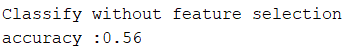
\includegraphics[width=0.4\linewidth]{../exercise3_1/images/classify_without_feature_selection.png}
		\caption{Αποτελέσματα από τo console της Matlab}
	\end{figure}
\subsection*{Classification with feature selection inside the cross validation}
	Στη δεύτερη περίπτωση δοκιμάσαμε να κάνουμε feature selection με μια απλή μέθοδο με την οποία επιλέγουμε τα χαρακτηριστικά που έχουν καλύτερη συσχέτιση με τα labels των δεδομένων μας. Πιο συγκεκριμένα, με τη συνάρτηση similarityMeasure() που μας δώθηκε μετράμε την ομοιότητα μεταξύ των feature και των label χρησιμοποιώντας τους συντελεστές συσχέτισης Pearson. Έπειτα, παίρνουμε τα 100 χαρακτηριστικά που έχουν τη το μεγαλύτερο συντελεστή και σε συνδυασμό με το cross validation κάνουμε train και υπολογίζουμε το συνολικό accuracy του ταξινομητή μας. Αυτή η επίλογή των 100 καλύτερων χαρακτηριστικών γίνεται μέσα στο cross validation, δηλαδή επαναλαμβάνεται Ν φορές. \\
	
	\noindent
	Tο συνολικό accuracy του SVM ταξινομητή είναι περίπου 0.6 ή 60\%, γεγονός που είναι αναμενόμενο, καθώς τα εντελώς τυχαία χαρακτηριστικά που δημιουργήσαμε δεν μας δίνουν κάποια χρήσιμη πληροφορία για το εάν ένα άτομο έχει διαγωνστεί με αυτισμό ή είναι φυσιολογικό.
	\begin{figure}[h!]
		\centering
		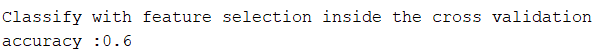
\includegraphics[width=0.7\linewidth]{../exercise3_1/images/classify_with_feature_selection_inside_cross_validation.png}
		\caption{Αποτελέσματα από τo console της Matlab}
	\end{figure}
\subsection*{Classification with feature selection outside the cross validation}
	Στη τρίτη και τελευταία περίπτωση κάνουμε πάλι την επιλογή χαρακτηριστικών που αναφέρθηκε στην προηγούμενη περίπτωση, με μοναδική διαφορά ότι αυτή η επιλογή χαρακτηριστικών γίνεται εκτός του cross validation, δηλαδή επαναλαμβάνεται 1 φορά. Τα αποτελέσματα που παίρνουμε σε αυτή την περίπτωση για το accuracy του SVM ταξινομητή είναι 1 ἠ 100\%, δηλαδή έχουμε το φαινόμενο του overfitting και ο ταξινομητής μας μας μαθαίνει πολύ καλά και με μεγάλη λεπτομέρεια τα training δεδομένα σε βαθμό που επηρεάζει την απόδοση του μοντέλου σε test δεδομένα. Αυτό σημαίνει ότι οι τυχαίες διακυμάνσεις στα δεδομένα εκπαίδευσης συλλέγονται και μαθαίνονται ως τάσεις από το μοντέλο.
	
	\begin{figure}[h!]
		\centering
		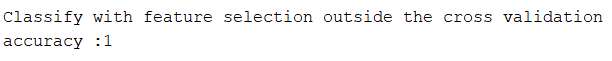
\includegraphics[width=0.7\linewidth]{../exercise3_1/images/classify_with_feature_selection_outside_cross_validation.png}
		\caption{Αποτελέσματα από τo console της Matlab}
	\end{figure}
\section*{Άσκηση 2: Υλοποίηση ενός απλού νευρωνικού δικτύου}
	Σε αυτή την άσκηση δημιουργήσαμε ένα απλό νευρωνικό δίκτυο το οποίο είχε μία είσοδο x και μία έξοδο y. To νευρωνικό δίκτυο που υλοποιήσαμε φαίνεται παρακάτω 
	
	\begin{figure}[h!]
		\centering
		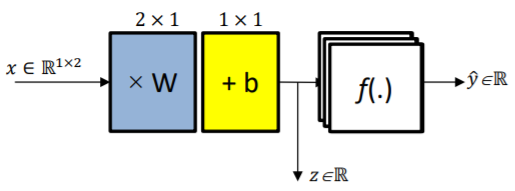
\includegraphics[height=4cm,width=0.5\linewidth]{../exercise3_2/python/images/simple_neural_network.png}
		\caption{Simple Neural Network}
	\end{figure}

	\noindent
	και ορίζεται από τη σχέση
	\begin{align*}
		\hat{y}^{(i)} &= f( x^{(i)} \cdot W + b )
	\end{align*}
	\noindent
	όπου $x^{(i)} \in \mathbb{R}^{1 \times 2}$ είναι ένα δείγμα, $W \in \mathbb{R}^{2 \times 1}$, $ b \in \mathbb{R}$ και $f(z) = \frac{1}{1 + e^{-z}}$
	
	\pagebreak
	\noindent
	To σφάλμα που υπάρχει ανάμεσα στην πρόβλεψη $hat{y}^{(i)}$ και στην τιμή $y^{(i)}$ που αντιστοιχεί στα δεδομένα $x^{(i)}$ μετριέται με τη συνάρτηση cross-entropy η οποία είναι η εξής
	\begin{align*}
		J(y^{(i)},\hat{y}^{(i)};W,b) = -y^{(i)} \cdot \ln(\hat{y}^{(i)}) - (1 - y^{(i)}) \cdot \ln(1 - \hat{y}^{(i)}) \tab \textit{σχέση (1)}
	\end{align*}
	
	\noindent
	Για να έχουμε αριθμητική ευστάθεια, υπολογίζουμε την cross-entropy για ένα σύνολο δειγμάτων Β (batch) και υπολογίσουμε το μέσο όρο 
	\begin{align*}
		J(Y,\hat{Y};W,b) = \frac{1}{B} \sum_{i} (-y^{(i)} \cdot \ln(\hat{y}^{(i)}) - (1 - y^{(i)}) \cdot \ln(1 - \hat{y}^{(i)})) \tab \textit{σχέση (2)}
	\end{align*}	

	\noindent
	Αν θέσουμε $ z^{(i)} = x^{(i)} \cdot W + b $, έχουμε $ \hat{y}^{(i)} = f(z^{(i)}) $ οπότε η μέση τιμή της συνάρτηση cross-entropy γίνεται 
	
	\begin{align*}
		J(Y,\hat{Y};W,b) &= \frac{1}{B} \sum_{i} \left(-y^{(i)} \cdot \ln\left(\hat{y}^{(i)}\right) - 
								\left(1 - y^{(i)}\right) \cdot \ln\left(1 - \hat{y}^{(i)}\right)\right) \\ 
						 &= \frac{1}{B} \sum_{i} \left(-y^{(i)} \cdot \ln\left(\frac{1}{1 + e^{-z^{(i)}}}\right) - 
						 		\left(1 - y^{(i)}\right) \cdot \ln\left(1 - \frac{1}{1 + e^{-z^{(i)}}}\right)\right) \\
						 &= \frac{1}{B} \sum_{i} \left(-y^{(i)} \cdot \ln\left(\frac{1}{1 + e^{-z^{(i)}}}\right) - 
						 		\left(1 - y^{(i)}\right) \cdot \ln\left(\frac{e^{-z^{(i)}}}{1 + e^{-z^{(i)}}}\right)\right) \\
						 &= \frac{1}{B} \sum_{i} \left(y^{(i)} \cdot \ln\left(1 + e^{-z^{(i)}}\right) - 
						 		\left(1 - y^{(i)}\right) \cdot \left(-z^{(i)}\right) + 
						 		\left(1 - y^{(i)}\right) \cdot \ln\left(1 + e^{-z^{(i)}}\right)\right) \\
						 &= \frac{1}{B} \sum_{i} \left(y^{(i)} \cdot \ln\left(1 + e^{-z^{(i)}}\right) + 
						 		 z^{(i)} - y^{(i)} \cdot z^{(i)} + 
						 		 \ln\left(1 + e^{-z^{(i)}}\right) - y^{(i)} \cdot \ln\left(1 + e^{-z^{(i)}}\right)\right) \\
						 &= \frac{1}{B} \sum_{i} \left(z^{(i)} - y^{(i)} \cdot z^{(i)} + 
						 		\ln\left(1 + e^{-z^{(i)}}\right)\right)
	\end{align*}
	\noindent
	Αν παραγωγίσουμε τη σχέση συνἀρτηση J ως προς $z^{(i)}$ έχουμε
	
	\begin{align*}
		\frac{\partial J(y^{(i)},\hat{y}^{(i)};W,b) }{\partial z^{(i)}} 
			&= \frac{\partial \left(z^{(i)} - y^{(i)} \cdot z^{(i)} + \ln\left(1 + e^{-z^{(i)}}\right)\right) }{\partial z^{(i)}} \\
		    &= 1 - y^{(i)} + \frac{-e^{-z^{(i)}}}{1 + e^{-z^{(i)}}} \\
		    &= -y^{(i)} + \frac{1}{1 + e^{-z^{(i)}}} \\
		    &= -y^{(i)} + f(z^{(i)}) \\
		    &= -y^{(i)} + \hat{y}^{(i)}, \tab \textit{όπου \ \ i} \in \textit{batch}
	\end{align*}
	
	\noindent
	Για τον υπολογισμό των $ \frac{\partial J }{ \partial W }$ και $ \frac{ \partial J }{ \partial b }$ έχουμε ότι η παράγωγος ενός αθροίσματος ισούται με το άθροισμα των παραγώνων. Οπότε για την πρώτη παράμετρο προκύπτει
	\begin{align*}
		\frac{\partial J(Y,\hat{Y};W,b) }{\partial W} 
				&= \frac{\partial \left( \frac{1}{B} \sum_{i} \left(z^{(i)} - y^{(i)} \cdot z^{(i)} + \ln\left(1 + e^{-z^{(i)}}\right)\right) \right) }{\partial W}\\
				&= \frac{1}{B} \sum_{i} \frac{\partial \left(z^{(i)} - y^{(i)} \cdot z^{(i)} + 
					\ln\left(1 + e^{-z^{(i)}}\right)\right) }{\partial W}\\
				&= \frac{1}{B} \sum_{i} \left(\frac{\partial \left(z^{(i)} - y^{(i)} \cdot z^{(i)} + \ln\left(1 + e^{-z^{(i)}}\right)\right) }{\partial z^{(i)}} \cdot \frac{\partial z^{(i)} }{\partial W}\right)
	\end{align*}

	\begin{align*}
		\frac{\partial J(Y,\hat{Y};W,b) }{\partial W} 
				&= \frac{1}{B} \sum_{i} \left(\frac{\partial \left(z^{(i)} - y^{(i)} \cdot z^{(i)} + \ln\left(1 + e^{-z^{(i)}}\right)\right) }{\partial z^{(i)} } \cdot \frac{\partial \left( x^{(i)} \cdot W + b \right) }{\partial W}\right) \\
				&= \frac{1}{B} \sum_{i} \left( \left(-y^{(i)} + \hat{y}^{(i)} \right)\cdot x^{(i)^{T}}\right)\\
				&= \frac{1}{B} \cdot 
				\begin{bmatrix}
					-y^{(1)} + \hat{y}^{(1)} & -y^{(2)} + \hat{y}^{(2)} & \cdots & -y^{(B)} + \hat{y}^{(B)} 
				\end{bmatrix} \cdot 
				\begin{bmatrix}
					x^{(1)^{T}} \\
					x^{(2)^{T}} \\
					\vdots \\
					x^{(B)^{T}} 
				\end{bmatrix}\\
				&= \frac{1}{B} \cdot \frac{\partial J(Y,\hat{Y};W,b) }{\partial z} \cdot x^{T}
	\end{align*}

	\noindent
	Επιπλέον, για τη δεύτερη παράμετρο έχουμε
	\begin{align*}
			\frac{\partial J(Y,\hat{Y};W,b) }{\partial b}  
					&= \frac{\partial \left( \frac{1}{B} \sum_{i} \left(z^{(i)} - y^{(i)} \cdot z^{(i)} + \ln\left(1 + e^{-z^{(i)}}\right)\right) \right) }{\partial b}\\
					&= \frac{1}{B} \sum_{i} \left(\frac{\partial \left(z^{(i)} - y^{(i)} \cdot z^{(i)} + \ln\left(1 + e^{-z^{(i)}}\right)\right) }{\partial z^{(i)}} \cdot \frac{\partial z^{(i)} }{\partial b}\right) \\
					&= \frac{1}{B} \sum_{i} \left( \left(-y^{(i)} + \hat{y}^{(i)} \right) \cdot \frac{\partial \left( x^{(i)} \cdot W + b \right) }{\partial b}\right) \\
					&= \frac{1}{B} \sum_{i} \left( \left(-y^{(i)} + \hat{y}^{(i)} \right) \cdot 1 \right) \\
					&= \frac{1}{B} \sum_{i} \left (-y^{(i)} + \hat{y}^{(i)} \right)
	\end{align*}

	\noindent
	Όσον αφορά τη συνάρτηση forward, αυτό που κάνουμε είναι να πολλαπλασιάσουμε την είσοδο x του νευρωνικου δικτύου με τα βάρη W και στη συνέχεια, αφού προστεθεί και το bias b, το αποτέλεσμα που προκύπτει δίνεται ως είσοδος με τη συνάρτηση sigmoid, ενώ επιστρέφουμε το το αποτέλεσμά της. \\
	
	\noindent
	Kατόπιν, υπολογίζουμε την απώλεια μεταξύ της εξόδου y και της πρόβλεψης $\hat{y}$ χρησιμοποιώντας τη συνάρτηση το $cross\_entropy$, στην οποία υλοποιήθηκε η σχέση (1).\\
	
	\noindent
	Στη συνέχεια, στη συνάρτηση backward αυτό που υπολογίζουμε είναι τις παραγώγους τις συνάρτησης κόστους ως προς z, W και b, ενώ επιστρέφουμε τις παραμέτρους $ \frac{\partial J }{ \partial W }$ και $ \frac{ \partial J }{ \partial b }$.\\
	
	\noindent
	Τέλος,  στη συνάρτηση $update\_weights$ κάνουμε ανανέωση τα βάρη W και το bias b του νευρωνικού μας δικτύου χρησιμοποιώντας την τεχνική του gradient descent. \\
	
	\noindent
	Από την προσομοίωση του νευρωνικού δικτύου προκύπτει ότι για αριθμό epoch 55, η απώλεια πέφτει από περίπου 0.53261 στο 0.35443. Επιπλέον, χρησιμοποιήθηκε το trained model για να γίνει πρόβλεψη της πιθανότητας και αυτό που βλέπουμε είναι ότι για βαθμούς 45 και 85 η πιθανότητα είναι περίπου 0.5321 ή 53.21\%. Τέλος, το accuracy των trained examples του νευρωνικού μετά την πρόβλεψη είναι 0.89 ή 89\%, γεγονός που φαίνεται από το παρακάτω figure στο οποίο φαίνεται ότι 4 δείγματα της μπλε κλάσης έχουν προβλεφθεί ως δείγματα της κόκκινης κλάσης, ενώ 7 δείγματα της κόκκινης κλάσης έχουν προβλεφθεί ως δείγματα της μπλέ κλάσης, δηλαδή συνολικά σε 11 από τα 100 δείγματα η πρόβλεψη είναι λανθασμένη.
	
	\pagebreak
	\begin{figure}[h!]
		\centering
		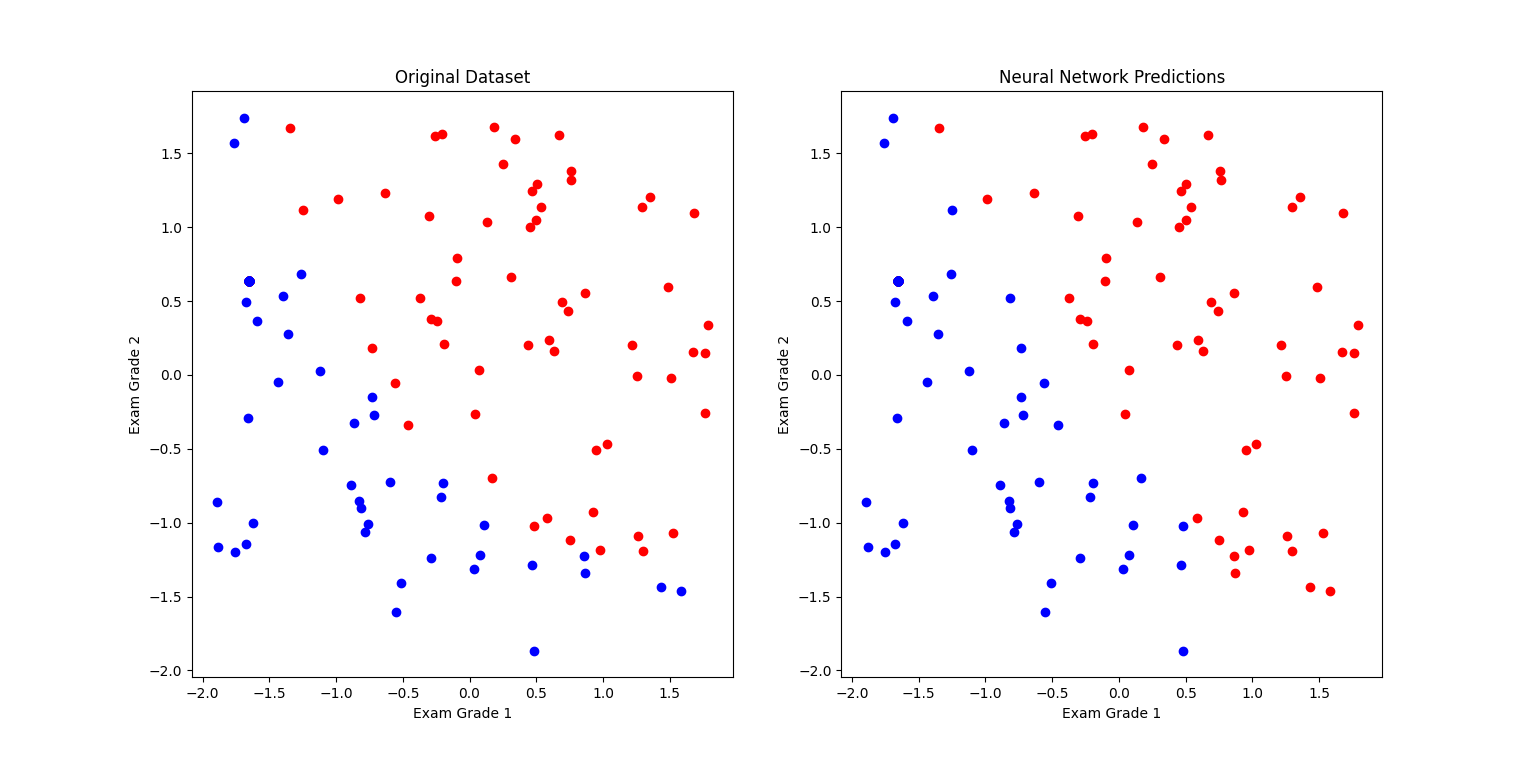
\includegraphics[height=7cm,width=\linewidth]{../exercise3_2/python/images/dataset_ANN_predictions.png}
		\caption{Dataset and neural network predictions - 55 Epochs}
	\end{figure}
	
	\noindent
	Αν αλλάξουμε τον αριθμό των epochs από 55 σε 400 θα παρατηρήσουμε ότι η απώλεια μειώνεται από περίπου 0.58489 σε 0.234561. Eιδικότερα, όσο περισσότερα epochs έχουμε τόσο μειώνεται η απώλεια του νευρωνικού δικτύου. Παράλληλα, η πιθανότητα για βαθμούς 45 και 85 αυξάνεται στο 0.6293 ή 62.93\%. Tἐλος, το συνολικό accuracy του νευρωνικού δικτύου αυξάνεται από 0.89 στο 0.9, όμως είναι μια πολύ μικρή αύξηση.
	
	\begin{figure}[h!]
		\centering
		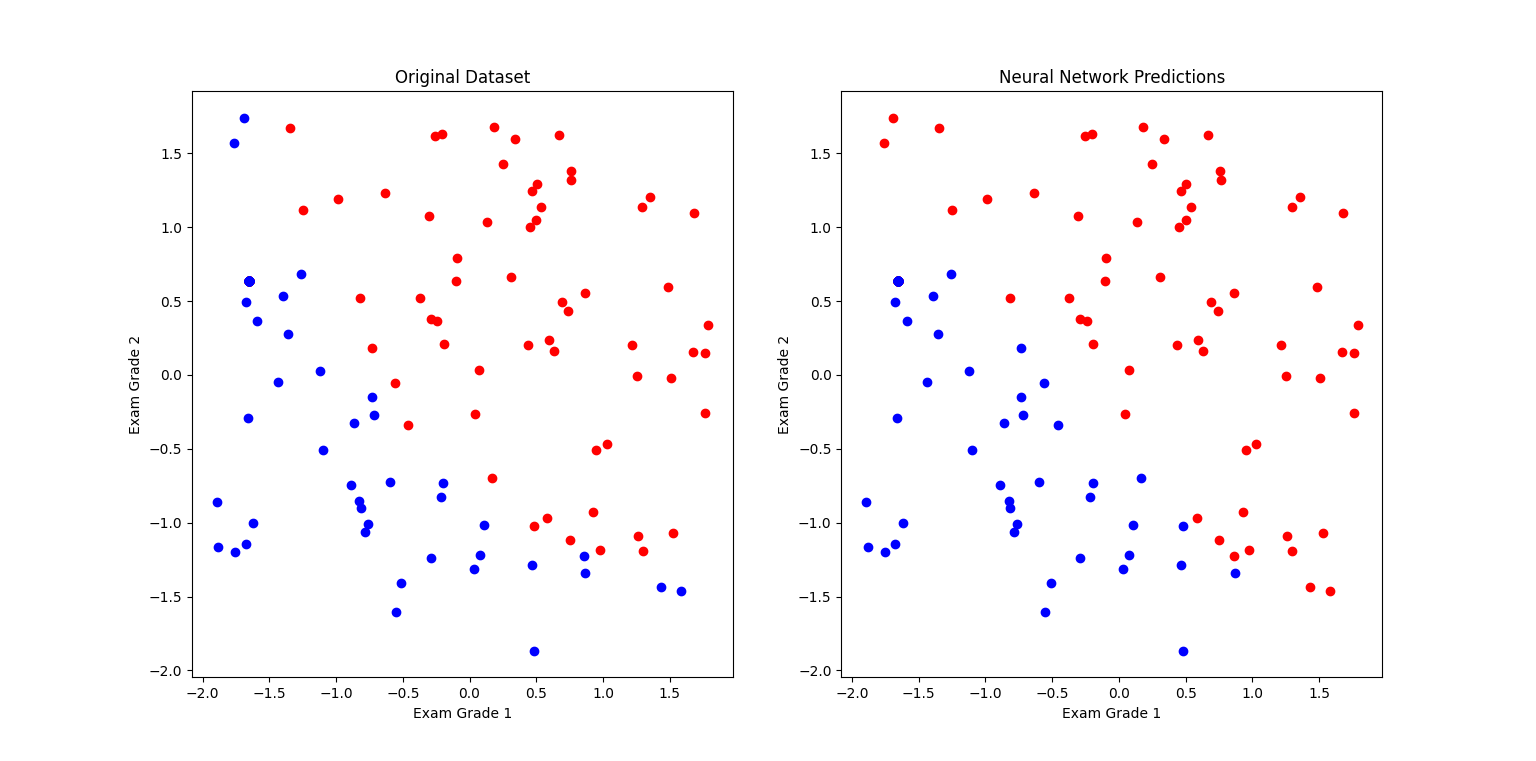
\includegraphics[height=7cm,width=\linewidth]{../exercise3_2/python/images/dataset_ANN_predictions_400_epochs.png}
		\caption{Dataset and neural network predictions - 400 Epochs}
	\end{figure}
\pagebreak
\section*{Άσκηση 3: Convolutional Neural Networks for Image Recognition}
	Σε αυτή την άσκηση δοκιμάσαμα διάφουρους ταξινομητές των νευρωνικών δικτύων χρησιμοποιώντας δεδομένα από τη βάση fashion-MNIST, η οποία περιέχει 10 κατηγορίες οι οποίες είναι T-shirt/top,
	Trouser, Pullover, Dress, Coat, Sandal, Shirt, Sneaker, Bag και Ankle boot. Πιο συγκεκριμένα μας δώθηκε ένα αρχείο fashion.py στο οποίο ήταν υλοποιημένος ένας ταξινομητής με dense νευρωνικό δίκτυο και δοκιμάσαμε με αριθμό epochs 400 να τρέξουμε το πρόγραμμα για κάποιους αλγορίθμους βελτιστοποίησης. Αυτοί οι αλγόριθμοι ήταν ο adam, sgd, rmsprop, nadam, adamax, και ftr. Τέλος, για κάθε μία περίπτωση αλγορίθμου βελτιστοποίησης τυπώσαμε κάποια δεδομένα πρόβλεψης και σε ένα άλλο διάγραμμα απεικονίσαμε το accuracy και validation accuracy συναρτήσει των epochs.
	\begin{figure}[h!]
		\centering
		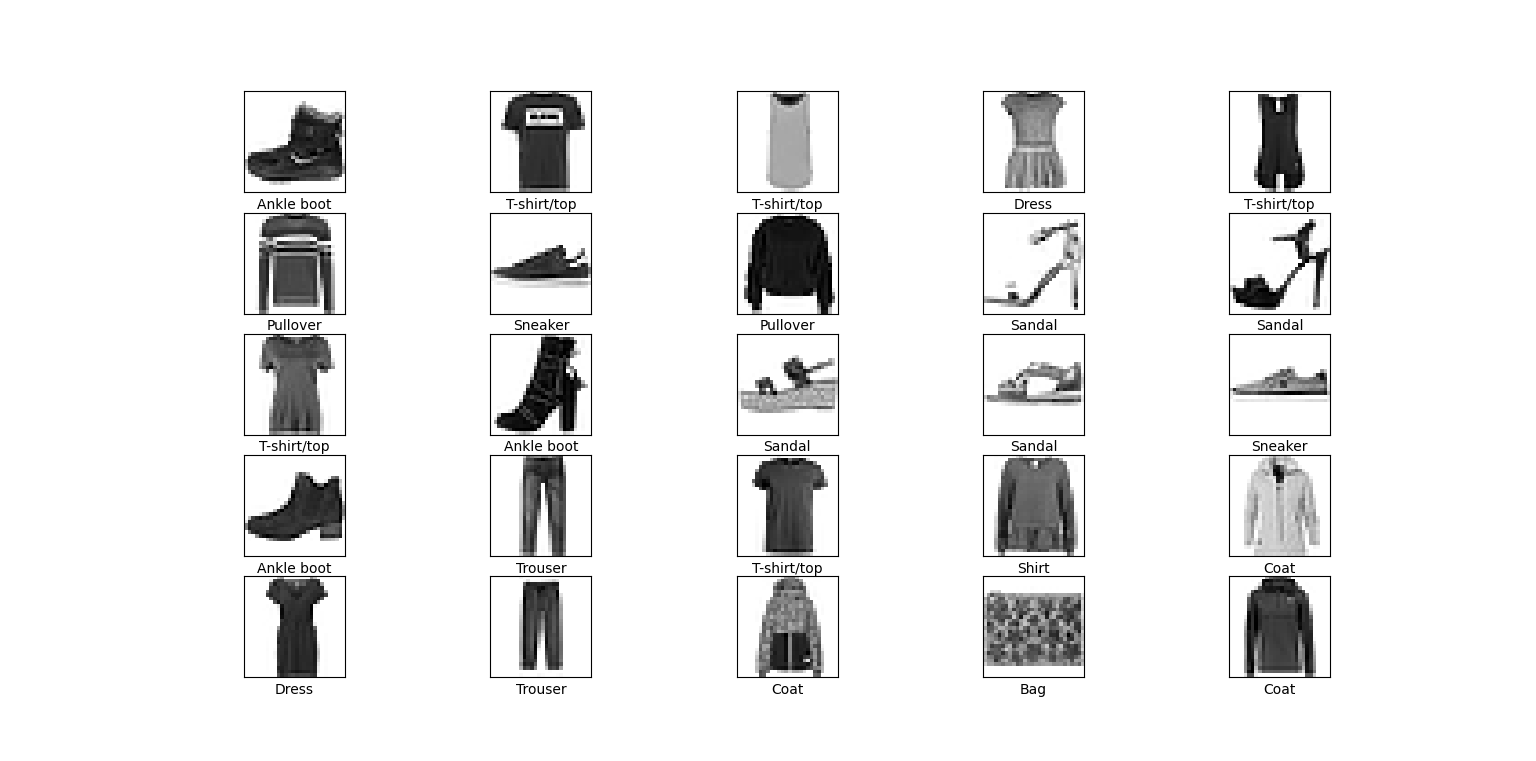
\includegraphics[height=7cm,width=\linewidth]{../exercise3_3/images/dataset.png}
		\caption{Initial Dataset}
	\end{figure}

\subsection*{Adam Optimizer}
	\begin{figure}[h!]
		\centering
		\begin{subfigure}[t]{0.5\textwidth}
			\centering
			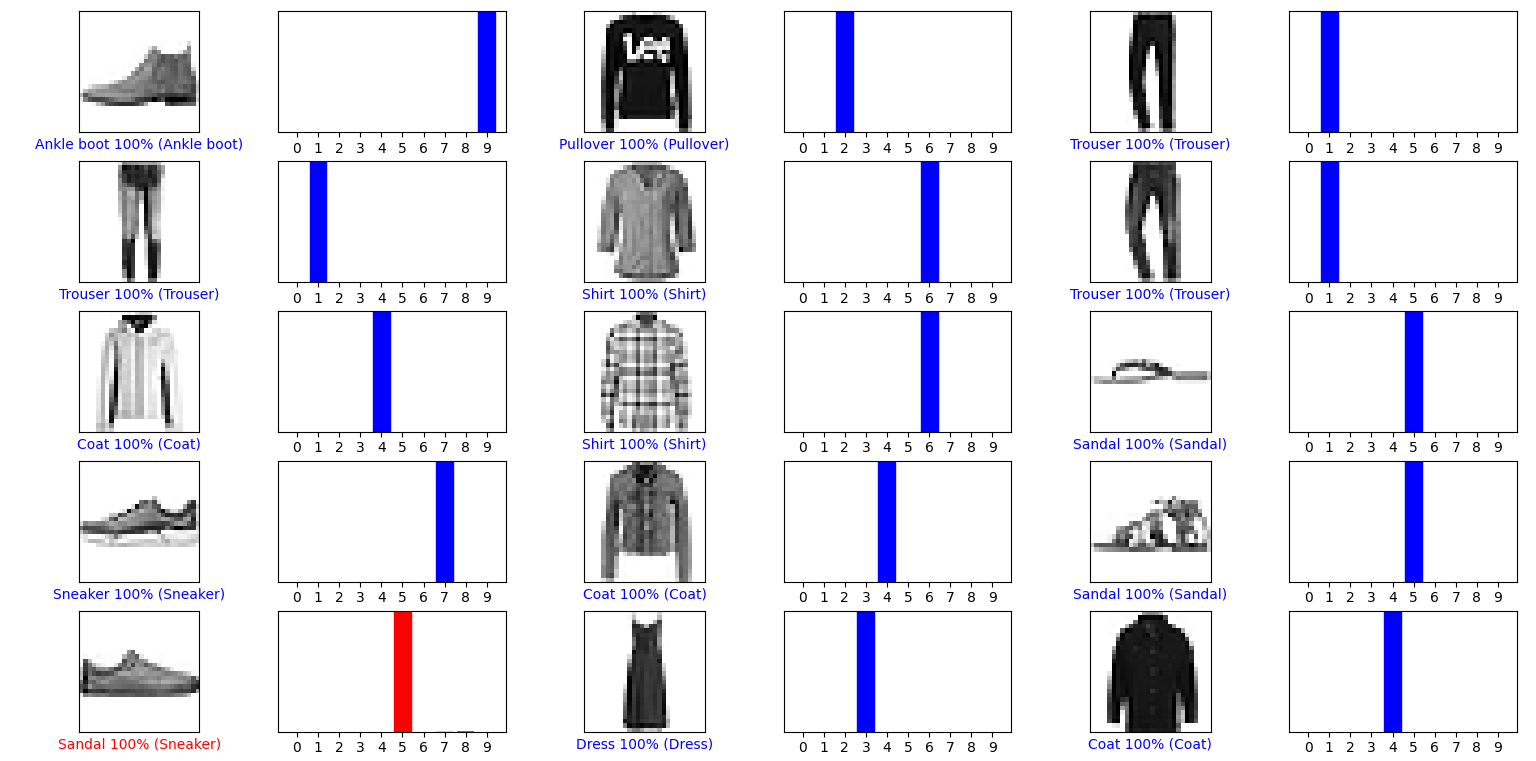
\includegraphics[width=\linewidth]{../exercise3_3/images/fashion_adam_probabilities.png}
			\caption{Adam Probabilities}
		\end{subfigure}%
		~
		\begin{subfigure}[t]{0.5\textwidth}
			\centering
			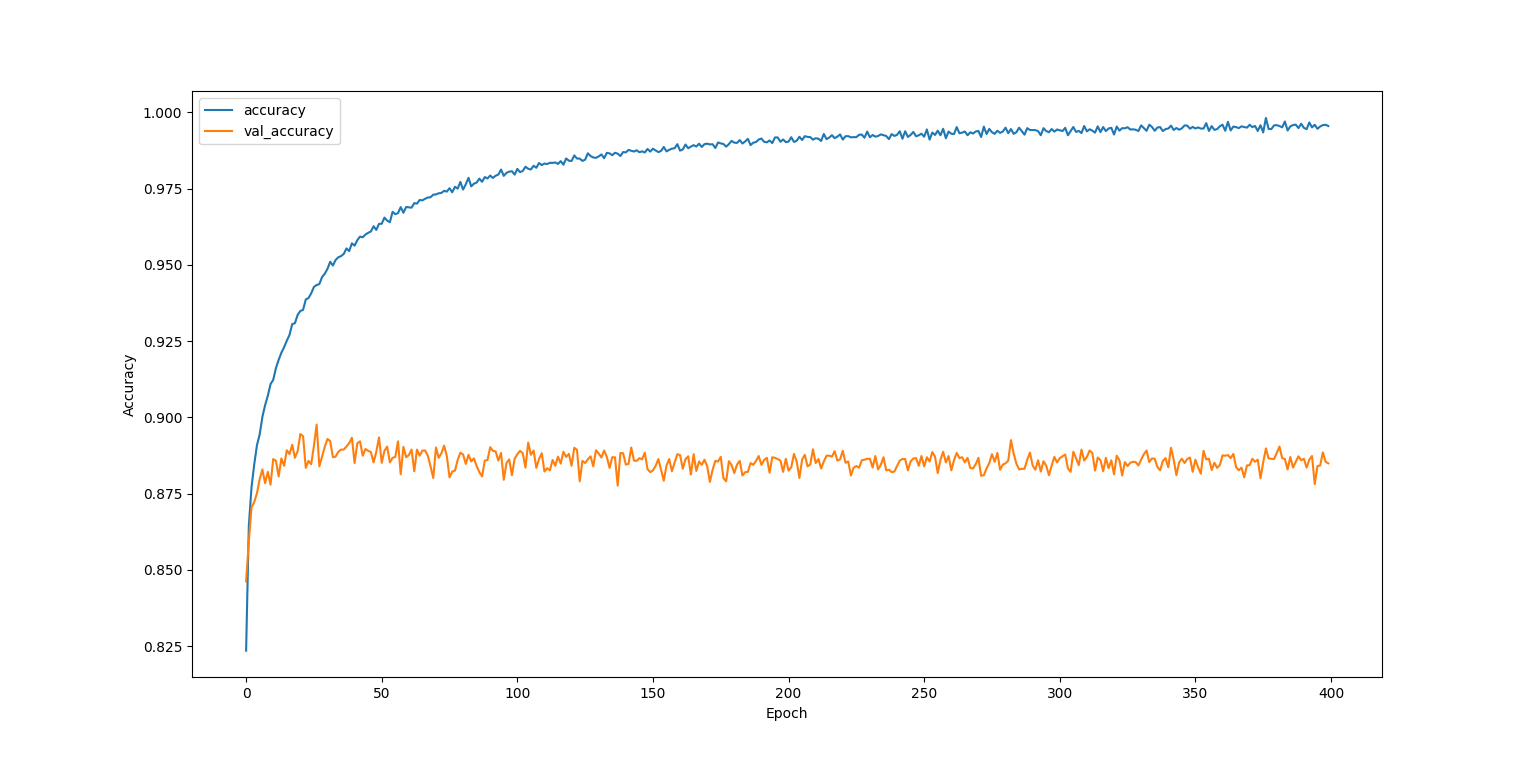
\includegraphics[width=\linewidth]{../exercise3_3/images/fashion_adam_accuracy.png}
			\caption{Adam Accuracy}
		\end{subfigure}
	\end{figure}
	\noindent
	\textbf{\underline{Aποτελέσματα του βελτιστοποιητή adam:}}\\
	Loss: 1.8922 \\
	Accuracy: 0.8849
	
\pagebreak
\subsection*{Sgd Optimizer}
		\begin{figure}[h!]
		\centering
		\begin{subfigure}[t]{0.5\textwidth}
			\centering
			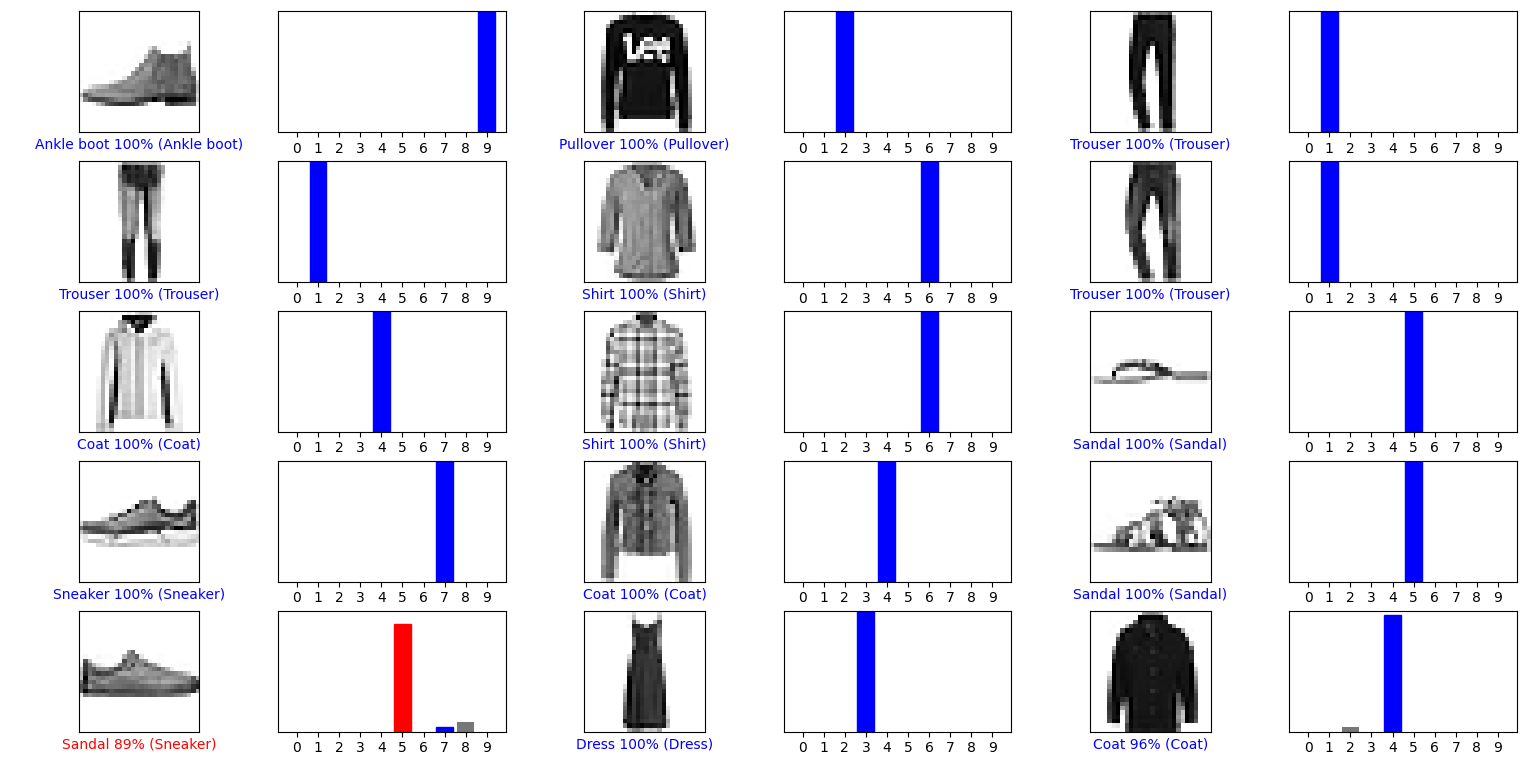
\includegraphics[width=\linewidth]{../exercise3_3/images/fashion_sgd_probabilities.png}
			\caption{Sgd Probabilities}
		\end{subfigure}%
		~
		\begin{subfigure}[t]{0.5\textwidth}
			\centering
			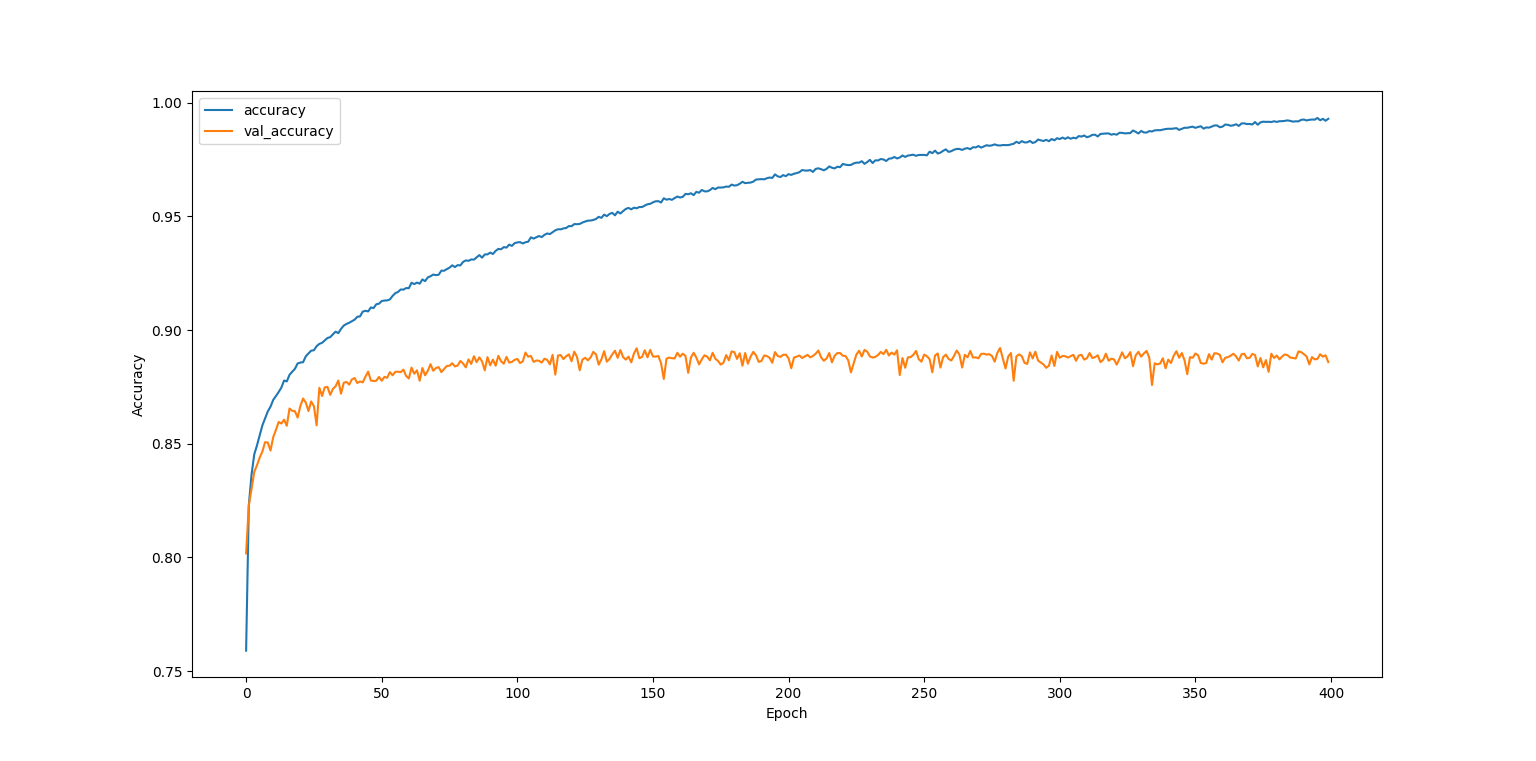
\includegraphics[width=\linewidth]{../exercise3_3/images/fashion_sgd_accuracy.png}
			\caption{Sgd Accuracy}
		\end{subfigure}
	\end{figure}
	\noindent
	\textbf{\underline{Aποτελέσματα του βελτιστοποιητή sgd:}}\\
	Loss: 0.5127 \\ 
	Accuracy: 0.8859

\subsection*{Rmsprop Optimizer}
	\begin{figure}[h!]
		\centering
		\begin{subfigure}[t]{0.5\textwidth}
			\centering
			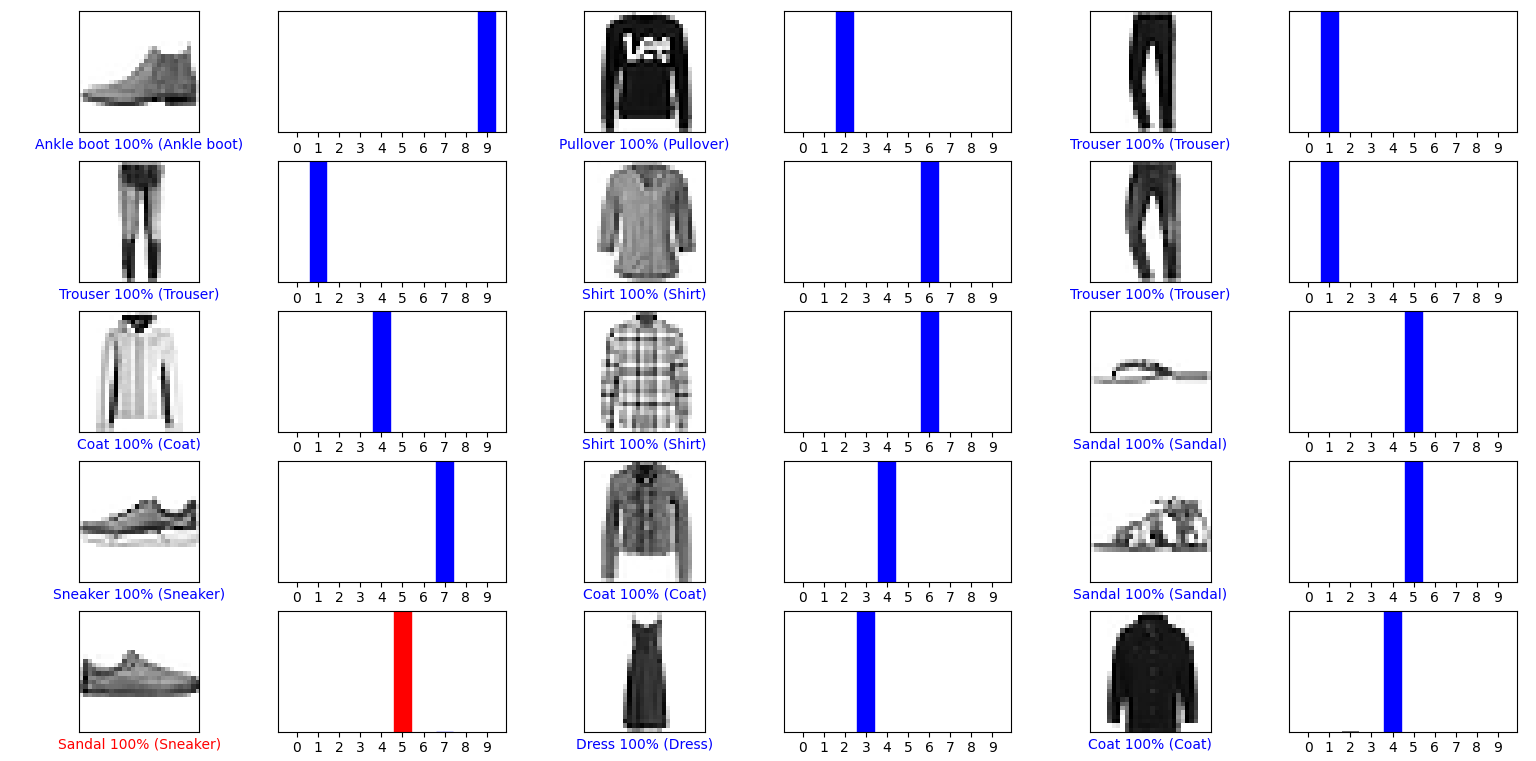
\includegraphics[width=\linewidth]{../exercise3_3/images/fashion_rmsprop_probabilities.png}
			\caption{Rmsprop Probabilities}
		\end{subfigure}%
		~
		\begin{subfigure}[t]{0.5\textwidth}
			\centering
			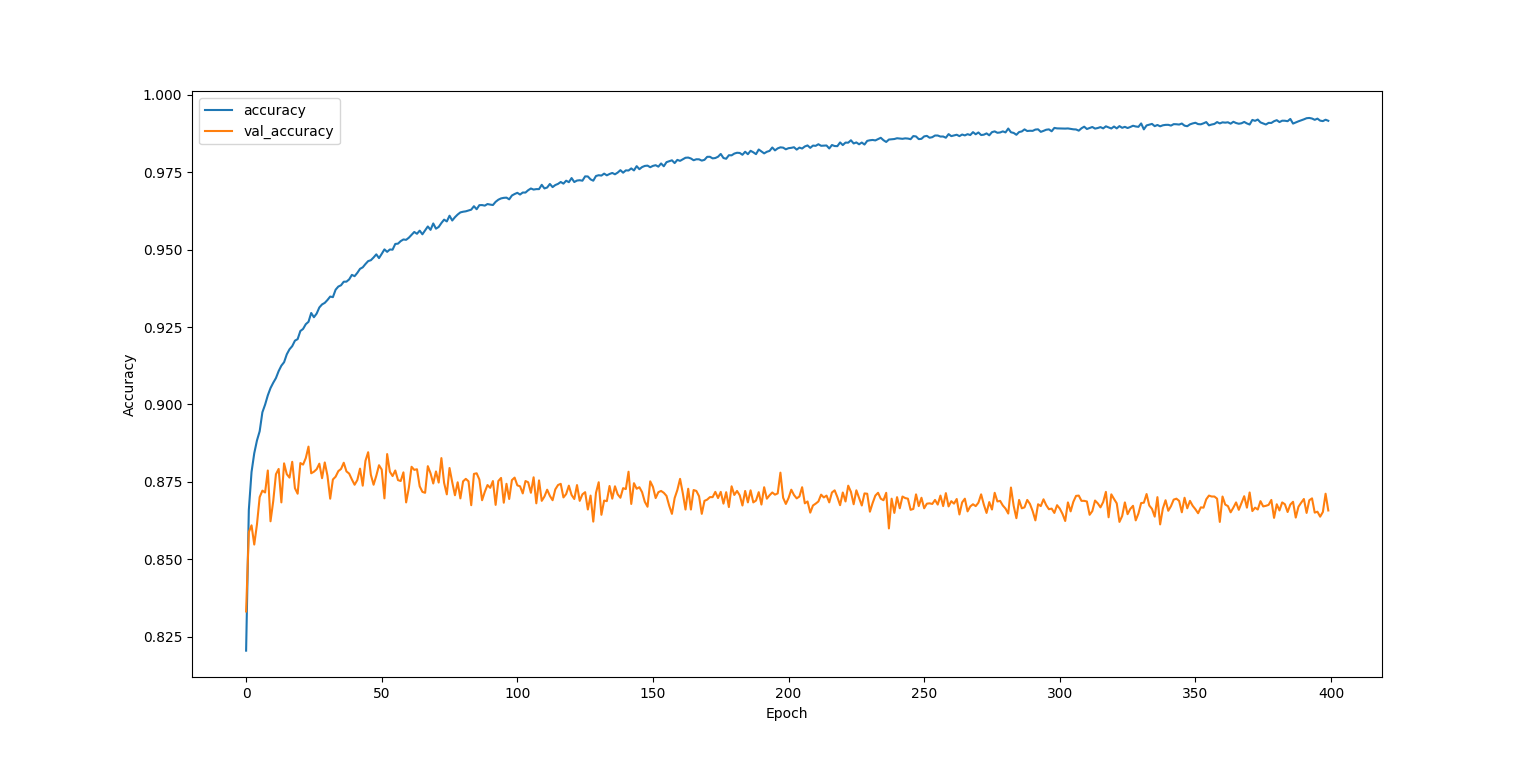
\includegraphics[width=\linewidth]{../exercise3_3/images/fashion_rmsprop_accuracy.png}
			\caption{Rmsprop Accuracy}
		\end{subfigure}
	\end{figure}
	\noindent
	\textbf{\underline{Aποτελέσματα του βελτιστοποιητή rmsprop:}}\\
	Loss: 4.4947 \\ 
	Accuracy: 0.8658
	
\subsection*{Nadam Optimizer}
	\begin{figure}[h!]
		\centering
		\begin{subfigure}[t]{0.5\textwidth}
			\centering
			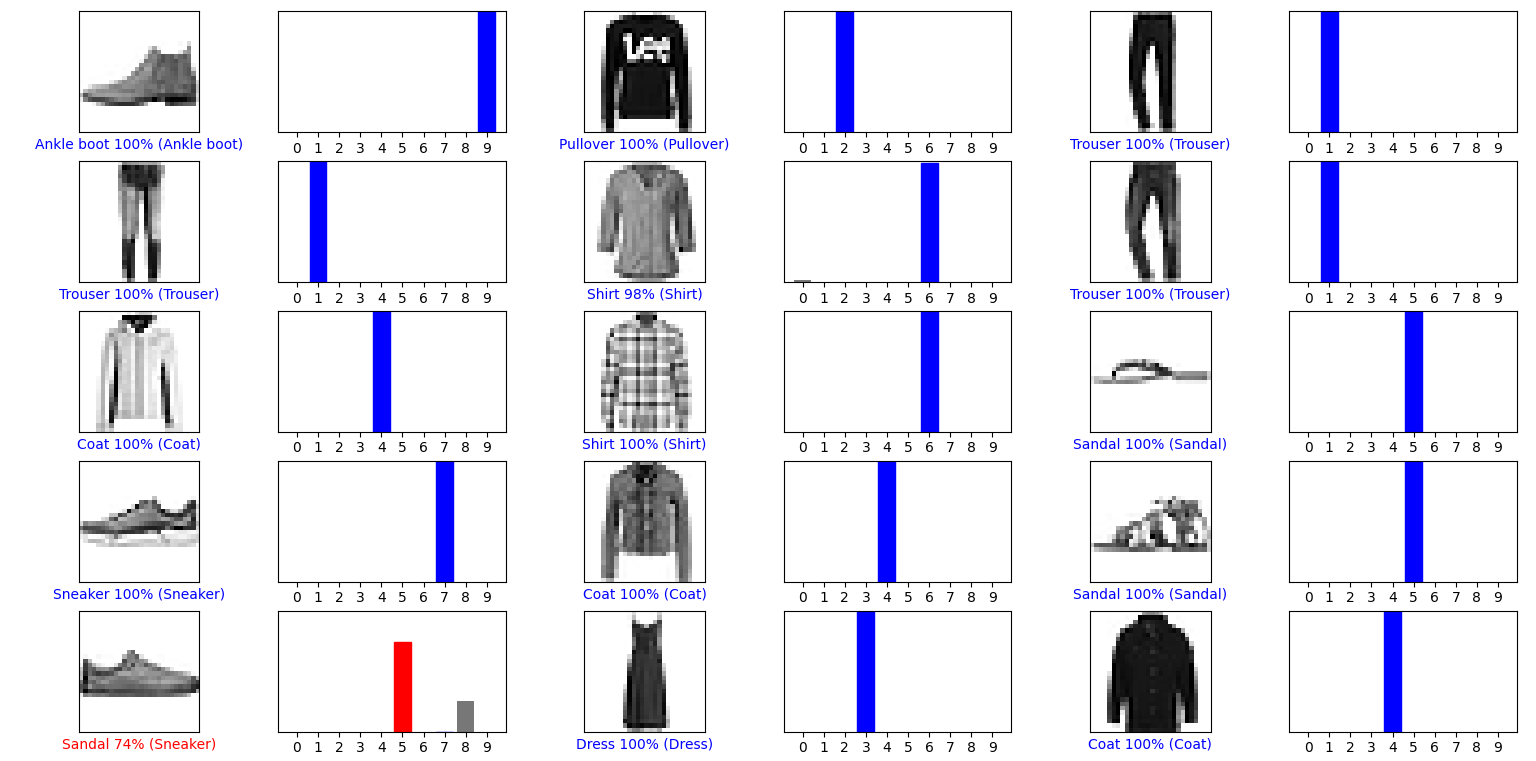
\includegraphics[width=\linewidth]{../exercise3_3/images/fashion_nadam_probabilities.png}
			\caption{Nadam Probabilities}
		\end{subfigure}%
		~
		\begin{subfigure}[t]{0.5\textwidth}
			\centering
			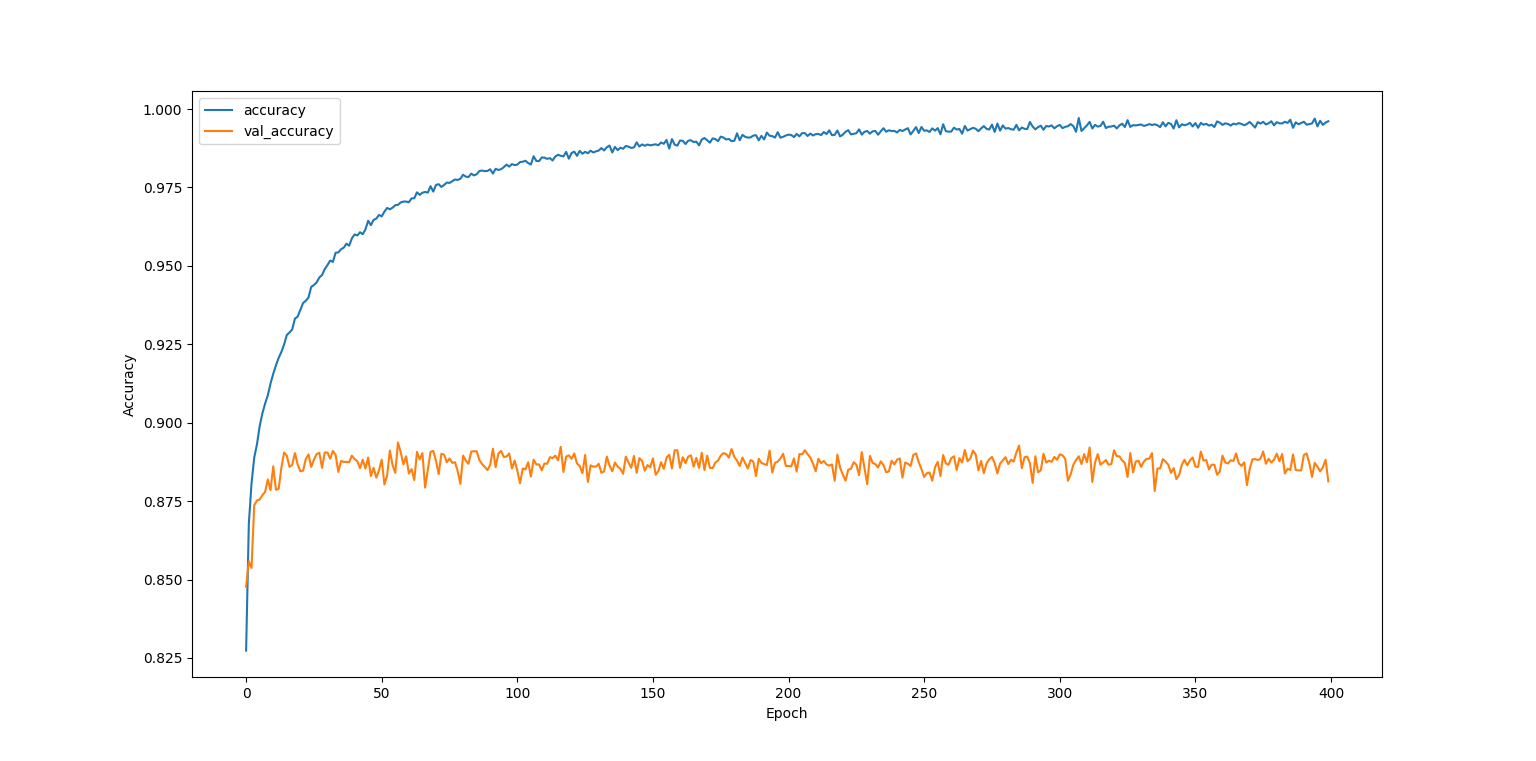
\includegraphics[width=\linewidth]{../exercise3_3/images/fashion_nadam_accuracy.png}
			\caption{Nadam Accuracy}
		\end{subfigure}
	\end{figure}
	\noindent
	\textbf{\underline{Aποτελέσματα του βελτιστοποιητή nadam:}}\\
	Loss: 1.9973 \\
	Accuracy: 0.8813

\pagebreak
\subsection*{Adamax Optimizer}
	\begin{figure}[h!]
		\centering
		\begin{subfigure}[t]{0.5\textwidth}
			\centering
			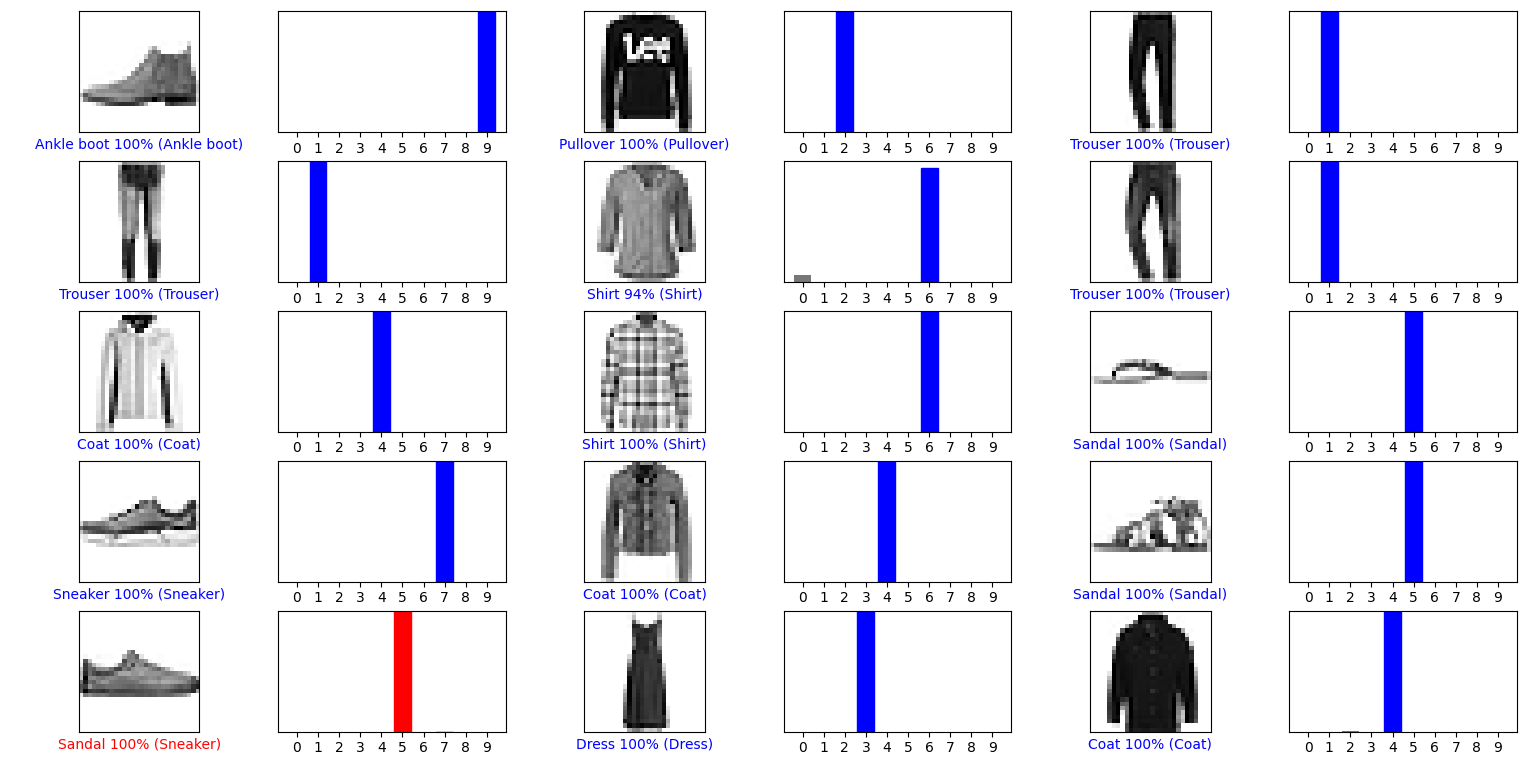
\includegraphics[width=\linewidth]{../exercise3_3/images/fashion_adamax_probabilities.png}
			\caption{Adamax Probabilities}
		\end{subfigure}%
		~
		\begin{subfigure}[t]{0.5\textwidth}
			\centering
			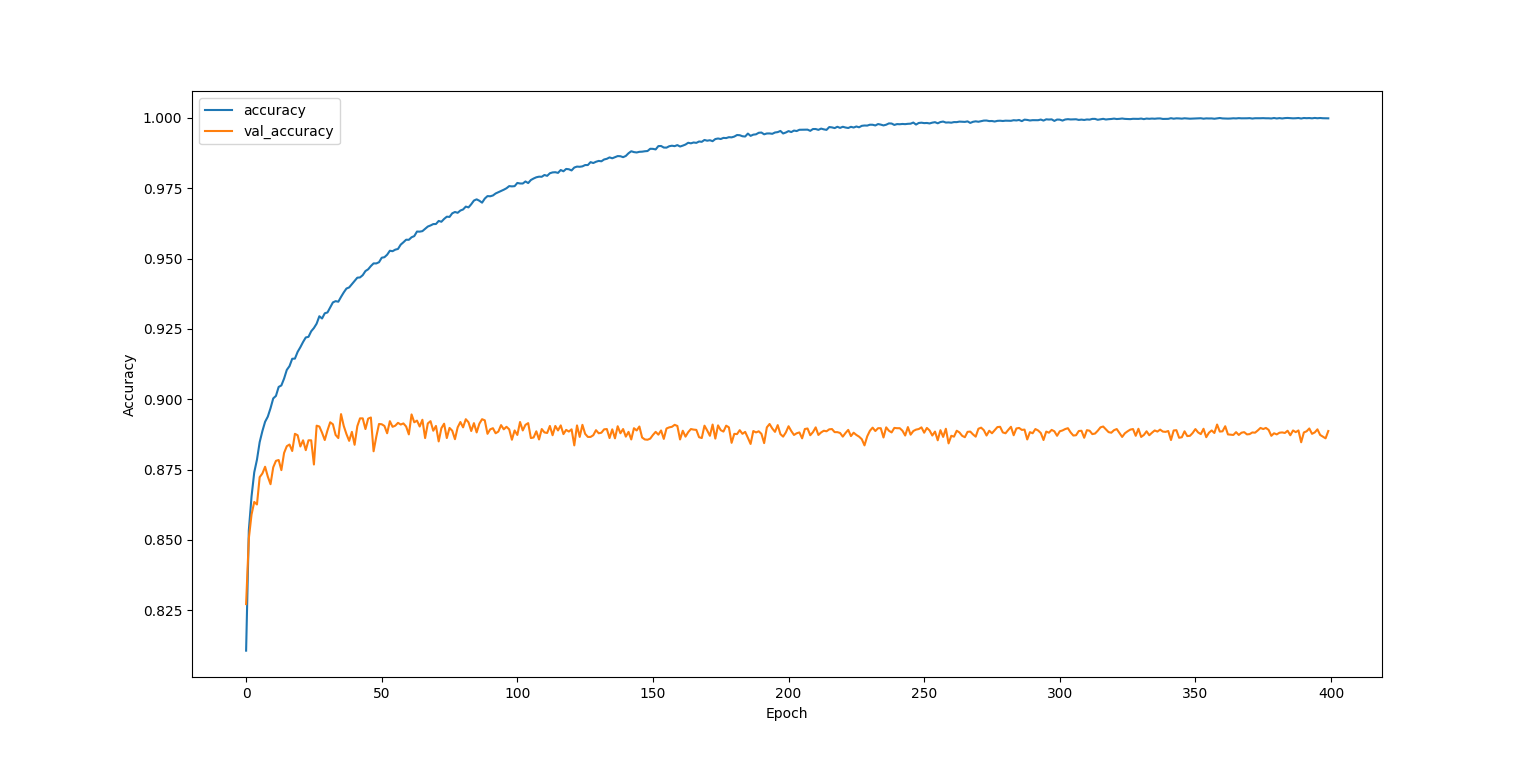
\includegraphics[width=\linewidth]{../exercise3_3/images/fashion_adamax_accuracy.png}
			\caption{Adamax Accuracy}
		\end{subfigure}
	\end{figure}
	\noindent
	\textbf{\underline{Aποτελέσματα του βελτιστοποιητή adamax:}}\\
	Loss: 0.9727 \\
	Accuracy: 0.8887
\subsection*{Ftrl Optimizer}
	\begin{figure}[h!]
		\centering
		\begin{subfigure}[t]{0.5\textwidth}
			\centering
			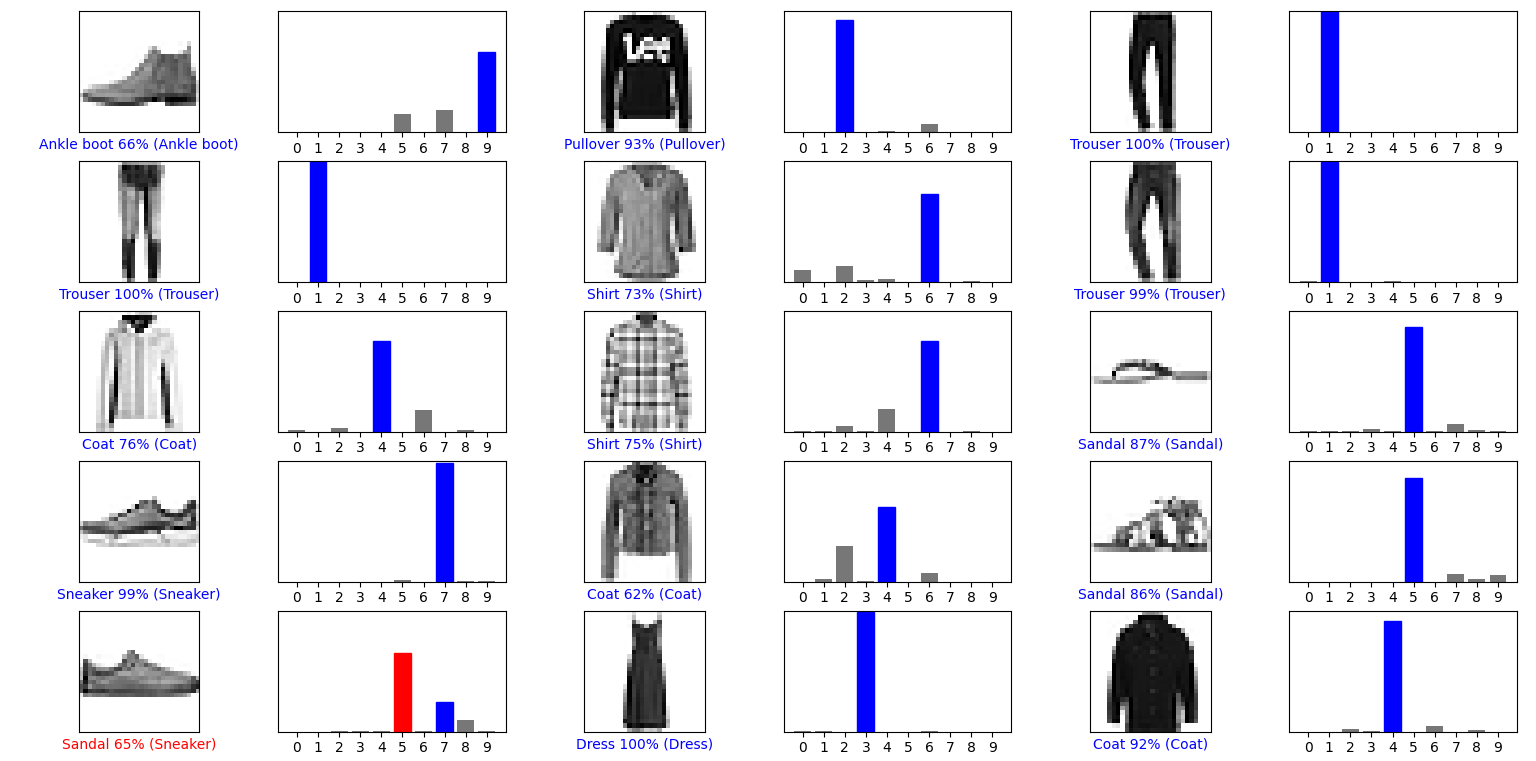
\includegraphics[width=\linewidth]{../exercise3_3/images/fashion_ftrl_probabilities.png}
			\caption{Adamax Probabilities}
		\end{subfigure}%
		~
		\begin{subfigure}[t]{0.5\textwidth}
			\centering
			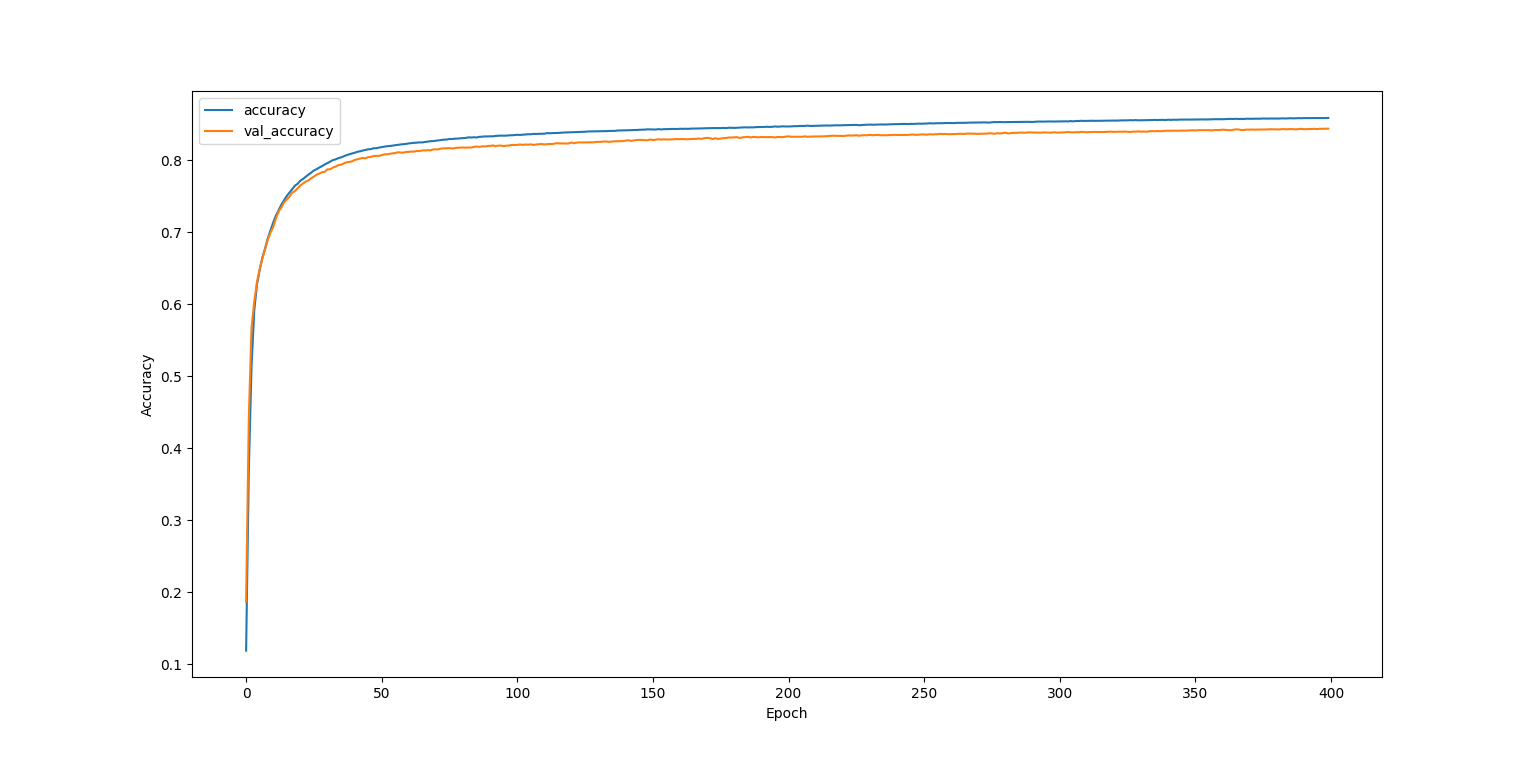
\includegraphics[width=\linewidth]{../exercise3_3/images/fashion_ftrl_accuracy.png}
			\caption{Adamax Accuracy}
		\end{subfigure}
	\end{figure}
	\noindent
	\textbf{\underline{Aποτελέσματα του βελτιστοποιητή ftrl:}}\\
	Loss: 0.4453 \\
	Αccuracy: 0.8440\\

	\noindent
	Αρχικά, αυτό που παρατηρούμε από τα διαγράμματα accuracy και validation accuracy συναρτήσει των epochs για τον αλγόριθμο βελτιστοποίησης adam είναι ότι το accuracy τείνει στη μονάδα, ενώ το validation είναι λίγο πάνω το 0.85 και ελάχιστα κάτω  από 0.9.\\
	 
	\noindent
	Παράλληλα, παρατηρώντας όλα τα παραπάνω αποτελέσματα, βλέπουμε ότι οι αλγόριθμοι που έχουν τα καλύτερα accuracy είναι ο adam, sgd, nadam και adamax. Πιο συγκεκριμένα, όλοι αυτοί οι αλγόριθμοι έχουν accuracy πάνω από 0.88, ενώ με πολύ μικρή διαφορά είναι είναι καλύτερος ο adamax. Ωστόσο, στον adamax παίρνει πολύ περισσότερο αριθμό epochs για να φτάσει σε αυτό το accuracy. Eπιπλεόν, παρατηρούμε ότι ο adam φτάνει στο accuracy του σε πολύ μικρότερο αριθμό epochs. Συνεπώς, επειδή τα accuracy αυτών των αλγορίθμων παρουσιάζουν ελάχιστες διαφορές και σε συνδυασμό με το γεγονός ότι ο adam φτάνει γρηγορότερα σε αυτό το accuracy, ο καταλληλότερος αλγόριθμος στο πρόβλημά μας είναι ο adam. \\
	
	\noindent
	Τέλος, όσον αφορά τους υπόλοιπους αλγορίθμους βλέπουμε ότι ο αμέσω καλύτερος αλγόριθμος με accuracy περίπου 0.8658 είναι ο rmsprop, ενώ ο χειρότερος αλγόριθμος βελτιστοποίησης για το πρόβλημά μας είναι ο ftrl, του οποίου το accuracy έιναι 0.844.\\


\subsection*{CNN with adam optimizer}
	\begin{figure}[h!]
		\centering
		\begin{subfigure}[t]{0.5\textwidth}
			\centering
			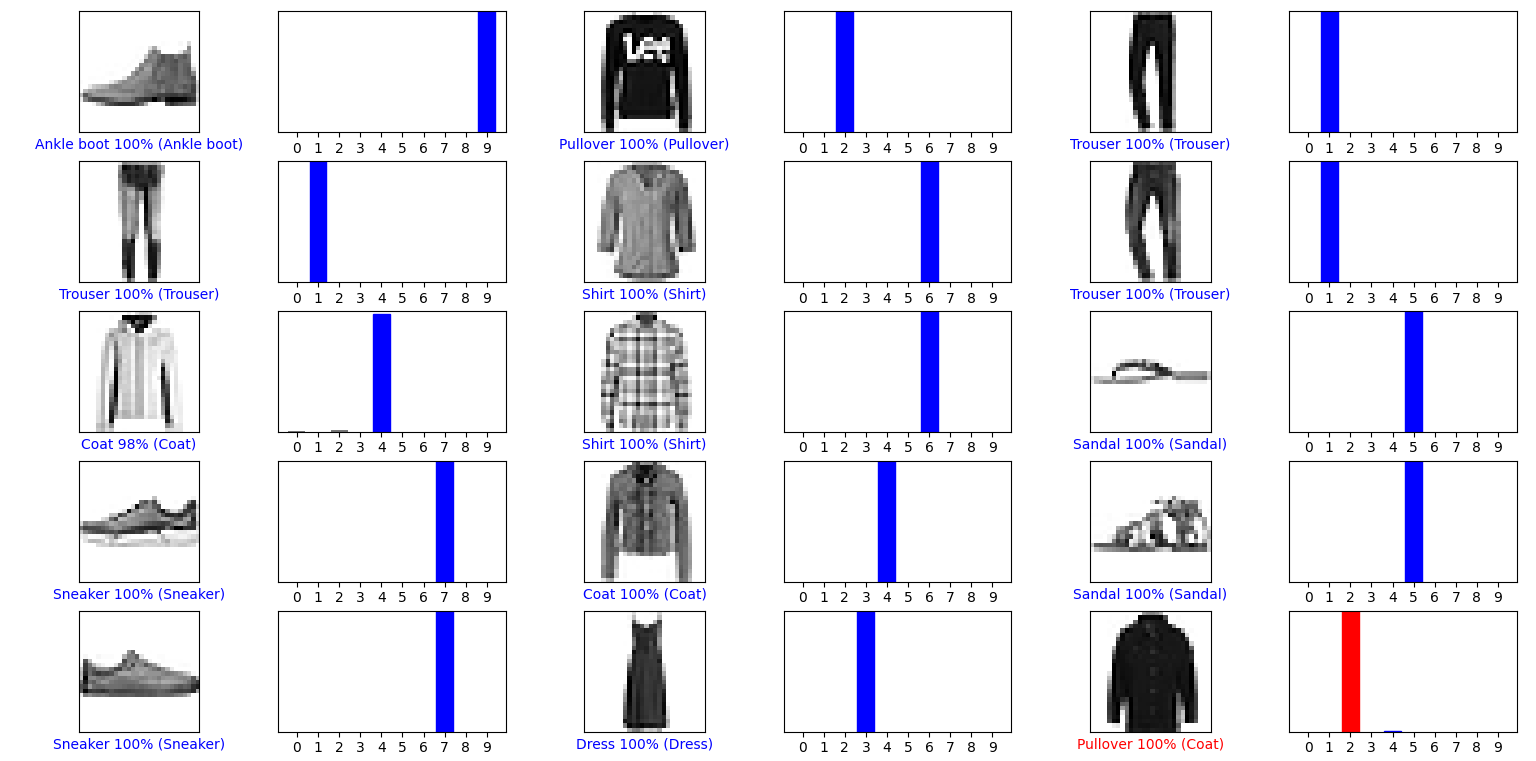
\includegraphics[width=\linewidth]{../exercise3_3/images/fashion_cnn_without_batch_relu_dropout_probabilities.png}
			\caption{Adam Probabilities}
		\end{subfigure}%
		~
		\begin{subfigure}[t]{0.5\textwidth}
			\centering
			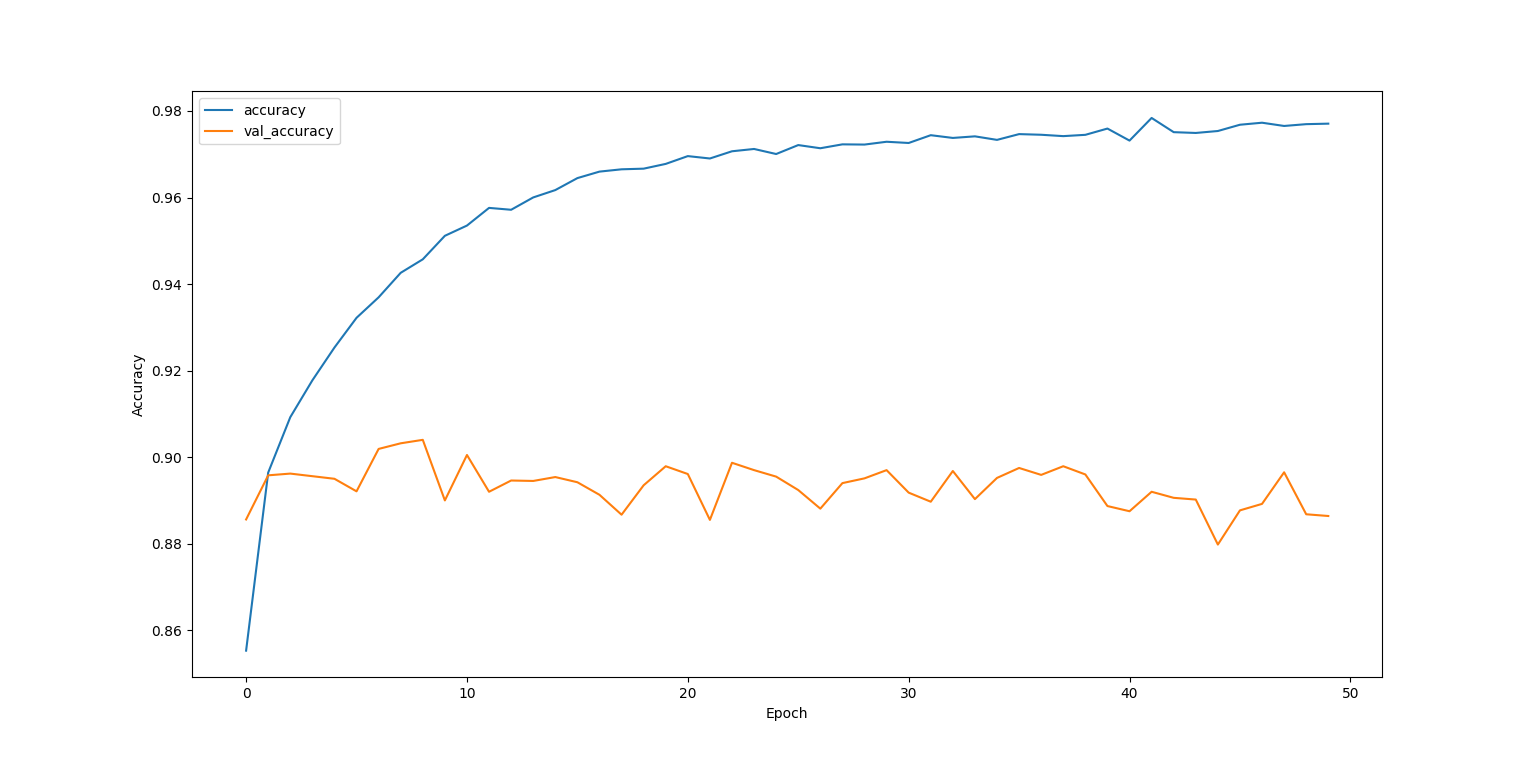
\includegraphics[width=\linewidth]{../exercise3_3/images/fashion_cnn_without_batch_relu_dropout_accuracy.png}
			\caption{Adam Accuracy}
		\end{subfigure}
		\caption{CNN - Without Batch Noramlization, Activation ReLU and Dropout}
	\end{figure}
	\noindent
	\textbf{\underline{Aποτελέσματα χωρίς Batch Normalization, Activation ReLU και Dropout:}}\\
	Loss: 1.1351 \\
	Accuracy: 0.8864
	
	\begin{figure}[h!]
		\centering
		\begin{subfigure}[t]{0.5\textwidth}
			\centering
			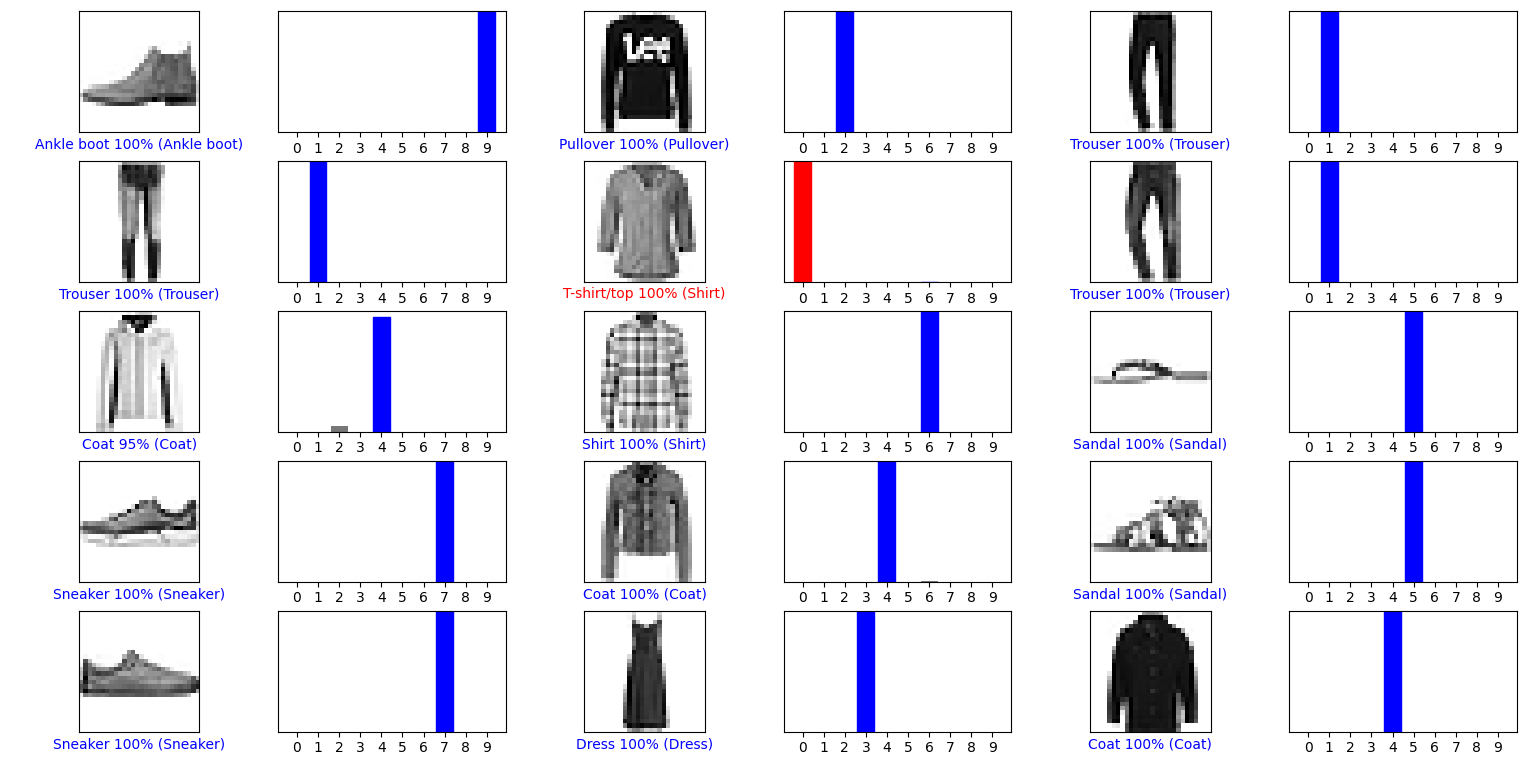
\includegraphics[width=\linewidth]{../exercise3_3/images/fashion_cnn_without_batch_dropout_probabilities.png}
			\caption{Adam Probabilities}
		\end{subfigure}%
		~
		\begin{subfigure}[t]{0.5\textwidth}
			\centering
			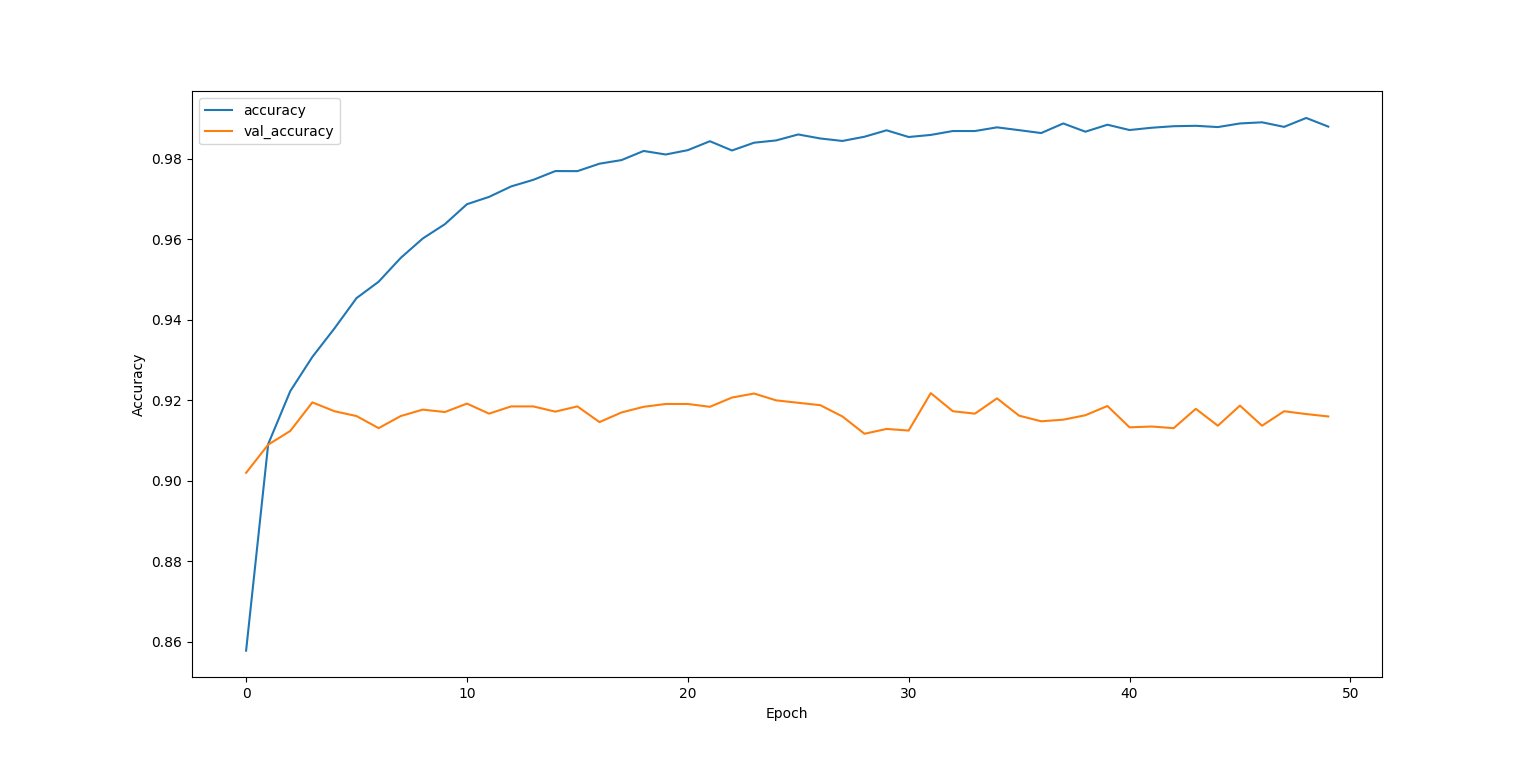
\includegraphics[width=\linewidth]{../exercise3_3/images/fashion_cnn_without_batch_dropout_accuracy.png}
			\caption{Adam Accuracy}
		\end{subfigure}
		\caption{CNN - With Activation ReLU, Without Batch Noramlization and Dropout}
	\end{figure}
	
	\noindent
	\textbf{\underline{Aποτελέσματα με Activation ReLU, χωρίς Batch Normalization και Dropout:}}\\
	Loss: 0.6968 \\
	Accuracy: 0.9160
	
	\begin{figure}[h!]
		\centering
		\begin{subfigure}[t]{0.5\textwidth}
			\centering
			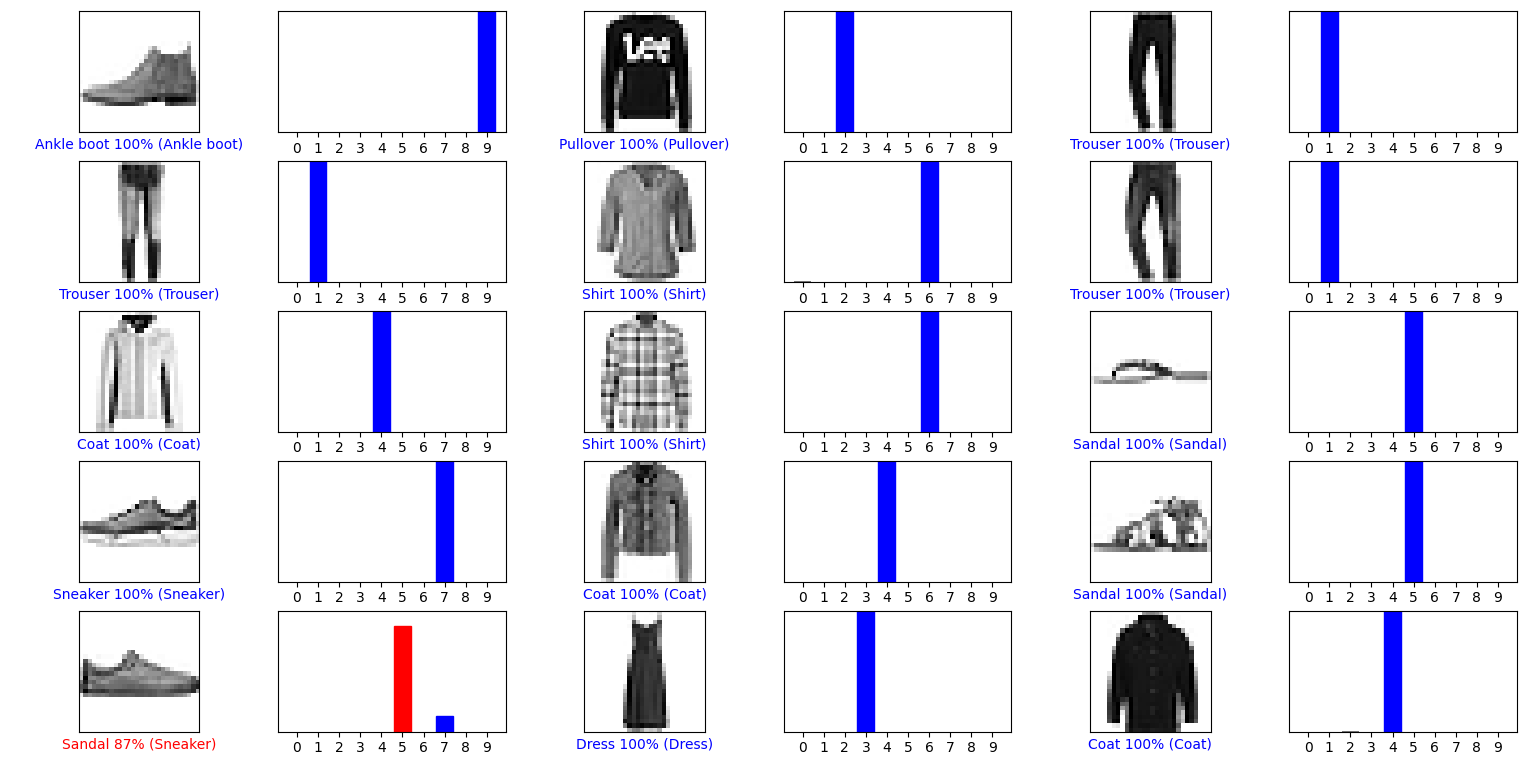
\includegraphics[width=\linewidth]{../exercise3_3/images/fashion_cnn_without_dropout_probabilities.png}
			\caption{Adam Probabilities}
		\end{subfigure}%
		~
		\begin{subfigure}[t]{0.5\textwidth}
			\centering
			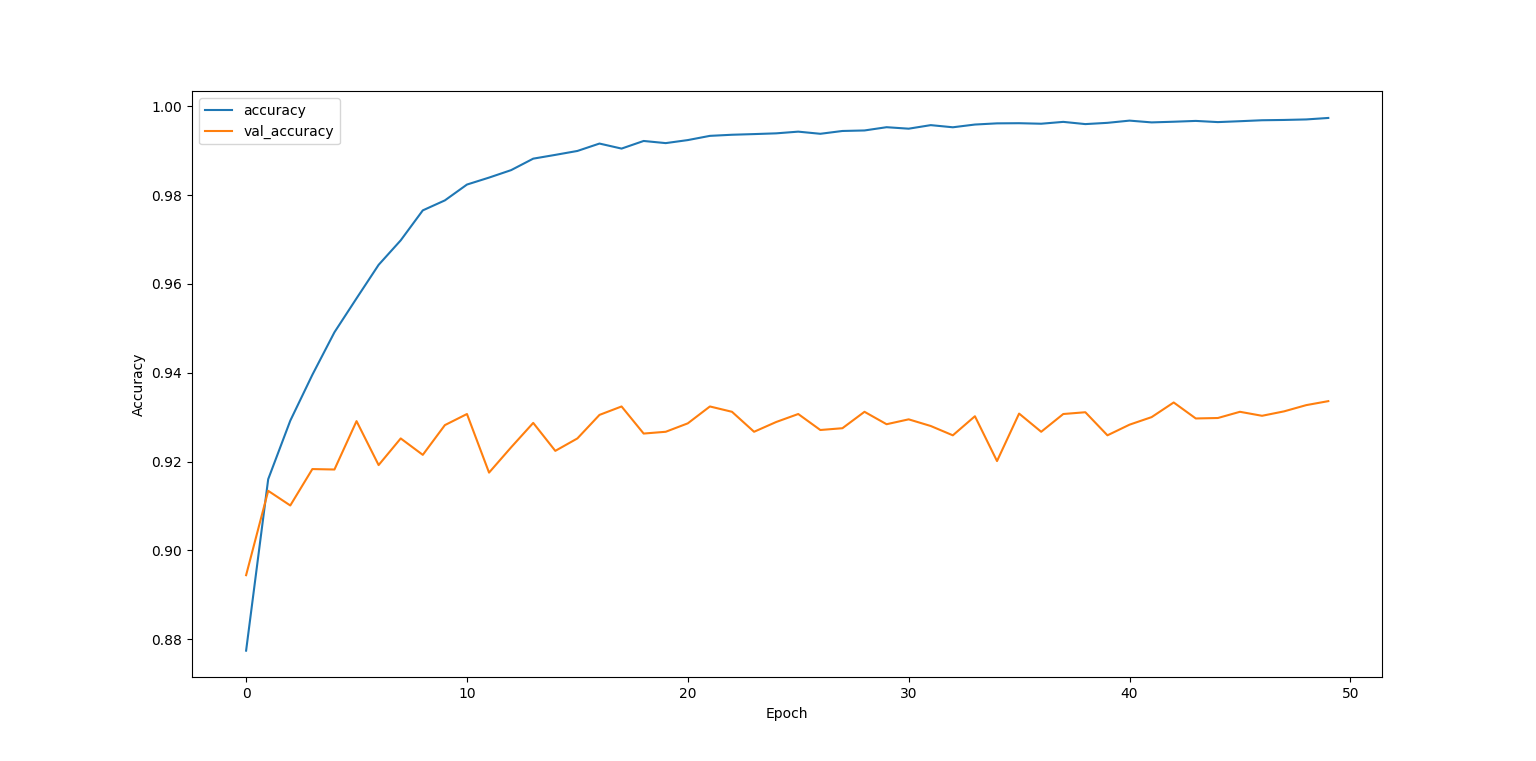
\includegraphics[width=\linewidth]{../exercise3_3/images/fashion_cnn_without_dropout_accuracy.png}
			\caption{Adam Accuracy}
		\end{subfigure}
		\caption{CNN - With Batch Noramlization, Activation ReLU, Without Dropout}
	\end{figure}
	\noindent
	\textbf{\underline{Aποτελέσματα με Batch Normalization, Activation ReLU, χωρίς Dropout:}}\\
	Loss: 0.4598 \\ 
	Accuracy: 0.9336
	
	\pagebreak
	\begin{figure}[h!]
		\centering
		\begin{subfigure}[t]{0.5\textwidth}
			\centering
			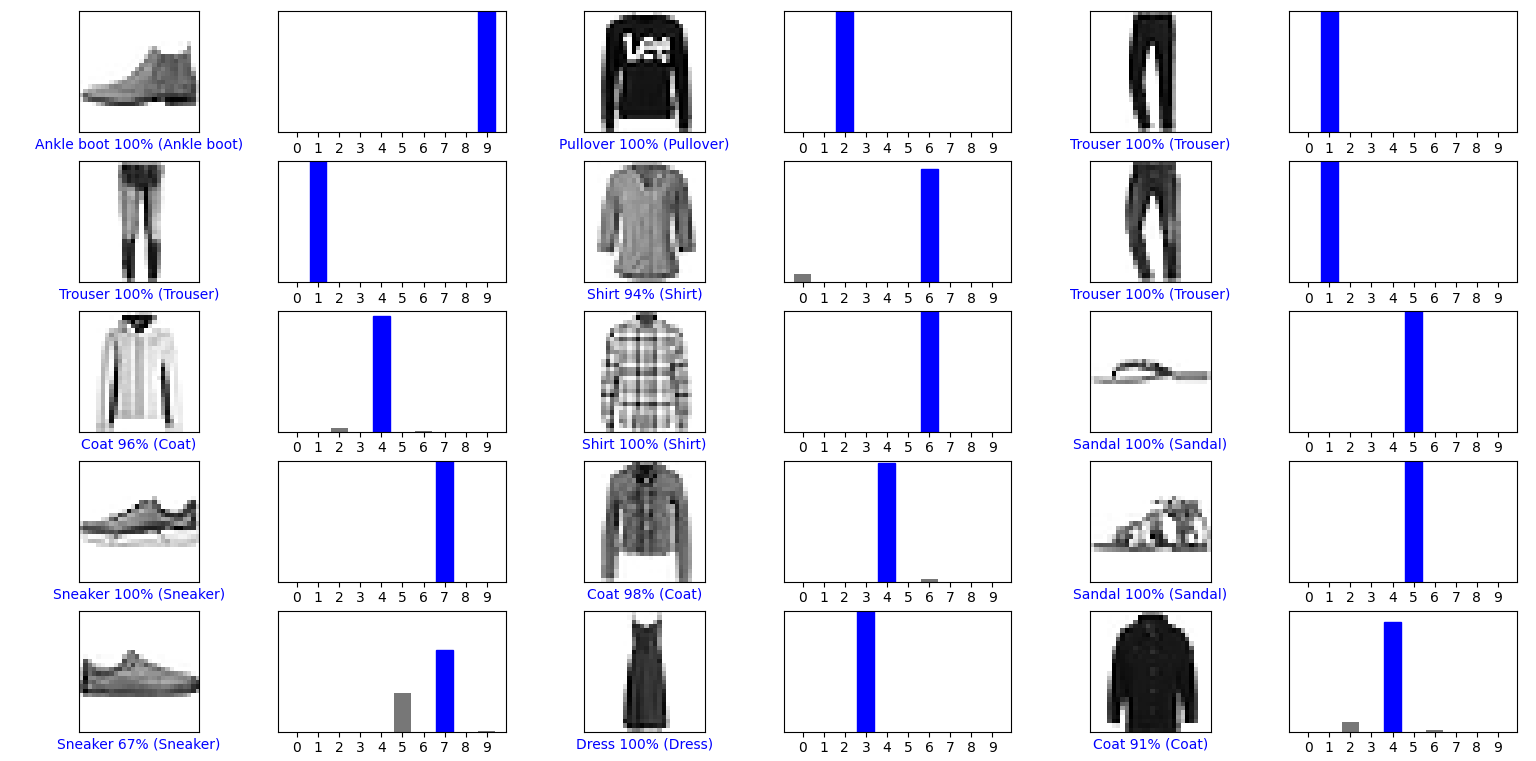
\includegraphics[width=\linewidth]{../exercise3_3/images/fashion_cnn_probabilities.png}
			\caption{Adam Probabilities}
		\end{subfigure}%
		~
		\begin{subfigure}[t]{0.5\textwidth}
			\centering
			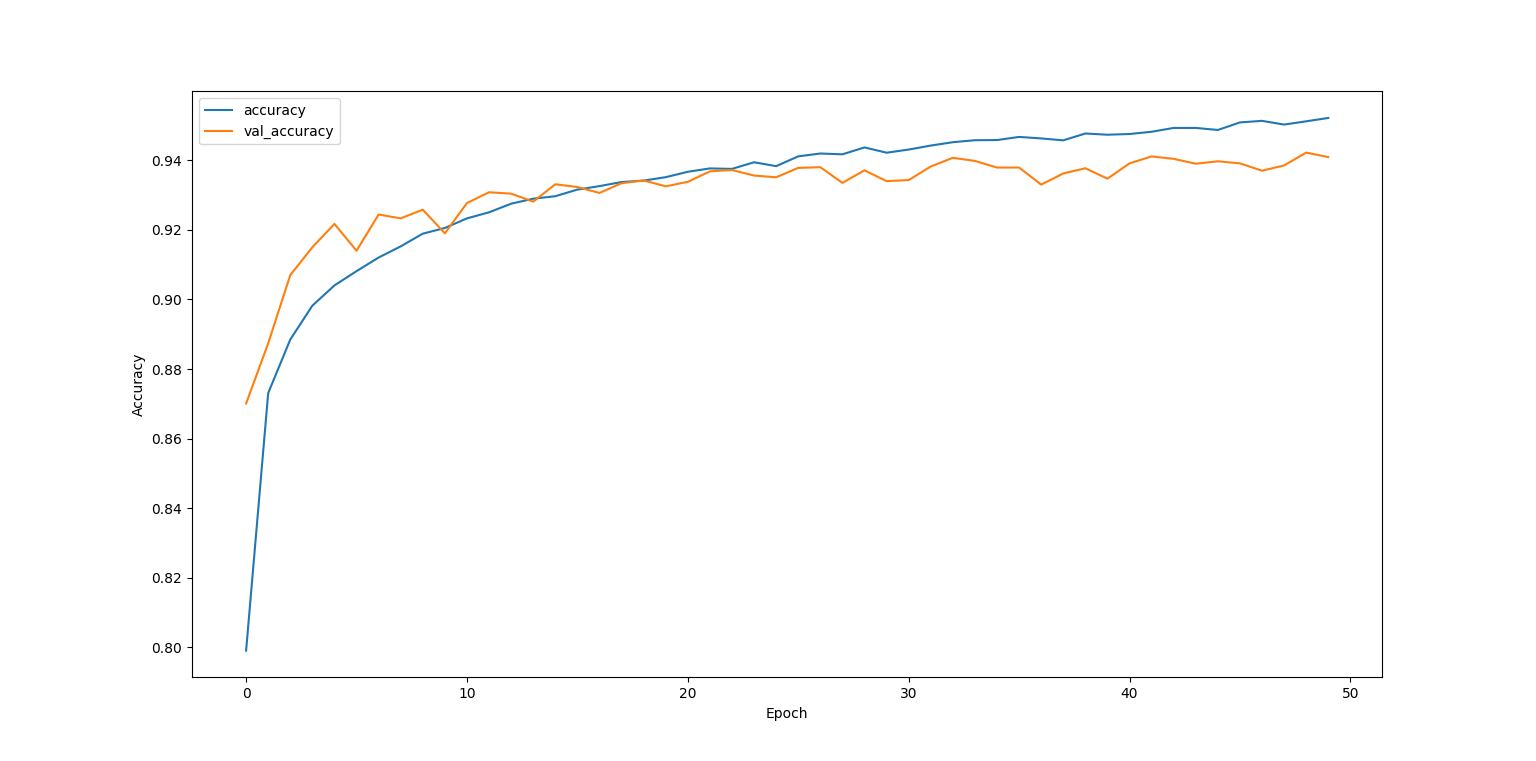
\includegraphics[width=\linewidth]{../exercise3_3/images/fashion_cnn_accuracy.png}
			\caption{Adam Accuracy}
		\end{subfigure}
		\caption{CNN - With Batch Normalization, Activation ReLU and Dropout}
	\end{figure}
	\noindent
	\textbf{\underline{Aποτελέσματα με Batch Normalization, Activation ReLU και Dropout:}}\\
	Loss: 0.1575 \\
	Αccuracy: 0.9409\\
	
	\noindent
	Όπως φαίνεται από τα παραπάνω διαγράμματα βλέπουμε ότι έχουμε τα χειρότερα αποτελέσματα, όταν δεν έχουμε κάποιο activation function, batch normalization και dropout. Ειδικότερα, έχουμε το μεγαλύτερο loss που κυμαίνεται περίπου στο 1.1351 και το μικρότερο accuracy περίπου στο 0.8864. \\
	
	\noindent
	Όταν χρησιμοποιούμε activation function ReLU, βλέπουμε ότι υπάρχει μια βελτίωση στα αποτελέσματα και το loss μειώνεται στο 0.6968, ενώ το accuracy αυτξάνεται στο 0,916. Παράλληλα, παρατηρούμε ότι ότα χρησιμοποιούμε batch normalization και στη συνέχεια activation function ReLU, έχουμε ακόμη καλύτερα αποτελέσματα και το loss μειώνεται στο 0.4598 και το accuracy αυξάνεται στο 0.9336.\\
	
	\noindent
	Με την ολοκλήρωση του νευρωνικού δικτύου και την προσθήκη dropout, έχουμε τα καλύτερα αποτελέσματα ως προς την αναγνώριση εικόνων. Το γεγονός αυτό φαίνεται και από το loss το οποίο είναι περίπου 0.1575, ενώ το accuracy γίνεται περίπου 0.9409, δηλαδή έχουμε το μικρότερο loos και το μεγαλύτερο accuracy από όλες τις παραπάνω περιπτώσεις.\\
	
	\noindent
	Τέλος, αυτό που παρατηρούμε από τα διαγράμματα accuracy και validation accuracy συναρτήσει των epochs, είναι ότι υπάρχει μία σύγκλισή τους καθώς πηγαίνουμε από τη μη χρήση batch normalization, activation function ReLU και dropout στη χρήση αυτών, δηλαδή το accuracy και validation accuracy τείνουν να ταυτιστούν.  
	
\end{document}
